% Options for packages loaded elsewhere
\PassOptionsToPackage{unicode}{hyperref}
\PassOptionsToPackage{hyphens}{url}
%
\documentclass[
  12pt,
]{book}
\usepackage{amsmath,amssymb}
\usepackage{lmodern}
\usepackage{setspace}
\usepackage{iftex}
\ifPDFTeX
  \usepackage[T1]{fontenc}
  \usepackage[utf8]{inputenc}
  \usepackage{textcomp} % provide euro and other symbols
\else % if luatex or xetex
  \usepackage{unicode-math}
  \defaultfontfeatures{Scale=MatchLowercase}
  \defaultfontfeatures[\rmfamily]{Ligatures=TeX,Scale=1}
\fi
% Use upquote if available, for straight quotes in verbatim environments
\IfFileExists{upquote.sty}{\usepackage{upquote}}{}
\IfFileExists{microtype.sty}{% use microtype if available
  \usepackage[]{microtype}
  \UseMicrotypeSet[protrusion]{basicmath} % disable protrusion for tt fonts
}{}
\makeatletter
\@ifundefined{KOMAClassName}{% if non-KOMA class
  \IfFileExists{parskip.sty}{%
    \usepackage{parskip}
  }{% else
    \setlength{\parindent}{0pt}
    \setlength{\parskip}{6pt plus 2pt minus 1pt}}
}{% if KOMA class
  \KOMAoptions{parskip=half}}
\makeatother
\usepackage{xcolor}
\IfFileExists{xurl.sty}{\usepackage{xurl}}{} % add URL line breaks if available
\IfFileExists{bookmark.sty}{\usepackage{bookmark}}{\usepackage{hyperref}}
\hypersetup{
  pdftitle={Entwicklung eines ML-basierten Tools zur Unterstützung der Bestimmung von Kornverteilungen in elektronenmikroskopischen Aufnahmen.},
  pdfauthor={Max Brede},
  hidelinks,
  pdfcreator={LaTeX via pandoc}}
\urlstyle{same} % disable monospaced font for URLs
\usepackage[left=4cm, right=3cm, top=2.5cm, bottom=2.5cm]{geometry}
\usepackage{longtable,booktabs,array}
\usepackage{calc} % for calculating minipage widths
% Correct order of tables after \paragraph or \subparagraph
\usepackage{etoolbox}
\makeatletter
\patchcmd\longtable{\par}{\if@noskipsec\mbox{}\fi\par}{}{}
\makeatother
% Allow footnotes in longtable head/foot
\IfFileExists{footnotehyper.sty}{\usepackage{footnotehyper}}{\usepackage{footnote}}
\makesavenoteenv{longtable}
\usepackage{graphicx}
\makeatletter
\def\maxwidth{\ifdim\Gin@nat@width>\linewidth\linewidth\else\Gin@nat@width\fi}
\def\maxheight{\ifdim\Gin@nat@height>\textheight\textheight\else\Gin@nat@height\fi}
\makeatother
% Scale images if necessary, so that they will not overflow the page
% margins by default, and it is still possible to overwrite the defaults
% using explicit options in \includegraphics[width, height, ...]{}
\setkeys{Gin}{width=\maxwidth,height=\maxheight,keepaspectratio}
% Set default figure placement to htbp
\makeatletter
\def\fps@figure{htbp}
\makeatother
\setlength{\emergencystretch}{3em} % prevent overfull lines
\providecommand{\tightlist}{%
  \setlength{\itemsep}{0pt}\setlength{\parskip}{0pt}}
\setcounter{secnumdepth}{1}
\newlength{\cslhangindent}
\setlength{\cslhangindent}{1.5em}
\newlength{\csllabelwidth}
\setlength{\csllabelwidth}{3em}
\newlength{\cslentryspacingunit} % times entry-spacing
\setlength{\cslentryspacingunit}{\parskip}
\newenvironment{CSLReferences}[2] % #1 hanging-ident, #2 entry spacing
 {% don't indent paragraphs
  \setlength{\parindent}{0pt}
  % turn on hanging indent if param 1 is 1
  \ifodd #1
  \let\oldpar\par
  \def\par{\hangindent=\cslhangindent\oldpar}
  \fi
  % set entry spacing
  \setlength{\parskip}{#2\cslentryspacingunit}
 }%
 {}
\usepackage{calc}
\newcommand{\CSLBlock}[1]{#1\hfill\break}
\newcommand{\CSLLeftMargin}[1]{\parbox[t]{\csllabelwidth}{#1}}
\newcommand{\CSLRightInline}[1]{\parbox[t]{\linewidth - \csllabelwidth}{#1}\break}
\newcommand{\CSLIndent}[1]{\hspace{\cslhangindent}#1}
\usepackage{booktabs}
\usepackage[ngerman]{babel}
\selectlanguage{ngerman}
\usepackage{subfig}
\usepackage{booktabs}
\usepackage{longtable}
\usepackage{array}
\usepackage{multirow}
\usepackage{wrapfig}
\usepackage{float}
\usepackage{colortbl}
\usepackage{pdflscape}
\usepackage{tabu}
\usepackage{threeparttable}
\usepackage{threeparttablex}
\usepackage[normalem]{ulem}
\usepackage{makecell}
\usepackage{xcolor}
\ifLuaTeX
  \usepackage{selnolig}  % disable illegal ligatures
\fi

\title{Entwicklung eines ML-basierten Tools zur Unterstützung der Bestimmung von Kornverteilungen in elektronenmikroskopischen Aufnahmen.}
\usepackage{etoolbox}
\makeatletter
\providecommand{\subtitle}[1]{% add subtitle to \maketitle
  \apptocmd{\@title}{\par {\large #1 \par}}{}{}
}
\makeatother
\subtitle{Thesis Beschreibung dies das.}
\author{Max Brede}
\date{2022-06-23}

\begin{document}
\maketitle

\renewcommand*\contentsname{Inhalt}
{
\setcounter{tocdepth}{1}
\tableofcontents
}
\listoffigures
\listoftables
\setstretch{1.5}
\hypertarget{einleitung}{%
\chapter{Einleitung}\label{einleitung}}

\hypertarget{motivation-und-problemstellung}{%
\section{Motivation und Problemstellung}\label{motivation-und-problemstellung}}

In der materialwissenschaftlichen Betrachtung von Werkstücken und deren Eignung für gegebene Anwendungsgebiete ist eine möglichst detaillierte Beschreibung und Charakterisierung derer Eigenschaften eine zentrale Voraussetzung. Je genauer ein Werkstück in seinen Eigenschaften beschrieben werden kann, desto besser kann das Verhalten untersucht und vorhergesagt werden(\protect\hyperlink{ref-askelandMaterialwissenschaftenGrundlagenUbungen1996}{Askeland, 1996}).

Diese Eigenschaften können in verschiedenen Größenordnungen bestimmt und zur Beantwortung unterschiedlicher Fragen genutzt werden.
Die erste mögliche Auflösung ist die Beschreibung der atomaren Zusammensetzung des Werkstücks, sowie dem Verhältnis verschiedener Atome zueinander, sollte mehr als ein Element enthalten sein. Aussagen auf dieser Ebene können zum Beispiel Auskunft über elektrische und magnetische Eigenschaften des Werkstücks ermöglichen (\protect\hyperlink{ref-askelandMaterialwissenschaftenGrundlagenUbungen1996}{Askeland, 1996}).
Als nächste Auflösungsstufe kann die Anordnung dieser Atome zueinander betrachtet werden. Diese meistens in einem Kristallgitter vorliegende Struktur kann Aussagen über zum Beispiel die Festigkeit eines Metalls liefern.
In einem Werkstück liegen verschiedene Kristalle in verschiedenen Gitterzusammensetzungen vor, die auch als Körner bezeichnet werden.
Der Verbund dieser Körner ist dann die nächste mögliche Betrachtungsebene, die auch als Mikrostruktur bezeichnet wird. Die Orientierung der Kristalle zueinander und in Bezug zur Ausrichtung des Werkstückes zusammen mit der Größe und Form der Kristallite spielt eine weitere große Rolle zum Beispiel im mechanischen Verhalten eines Materials.

Die Charakterisierung dieser Mikrostruktur ist die Aufgabe des Ausbildungsberufs des Metallographen. Diese Fachkräfte werden zum Beispiel in Stahlwerken eingesetzt, wo sie das Gefüge der im Material vorhandenen Kristalle durch Politur und Ätzung sichtbar machen. Diese Verfahren werden eingesetzt, um die Grenzen zwischen Körnern, die natürlicherweise Gitterfehler und damit Schwachpunkte des Materials darstellen, sichtbar zu machen. Da der Gitterverbund an diesen Grenzen schwächer ist, werden Atome hier leichter von Säuren ausgelöst, was zu einem mit einem Lichtmikroskop darstellbaren Höhenunterschied zwischen Korn und Korngrenze führt (\protect\hyperlink{ref-GefugeWerkstoffkunde2021}{{``Gefüge (Werkstoffkunde),''} 2021}). Ein Beispiel für ein so behandeltes Werkstück ist in Abbildung \ref{fig:baseGrain} zu sehen.





\begin{figure}

{\centering 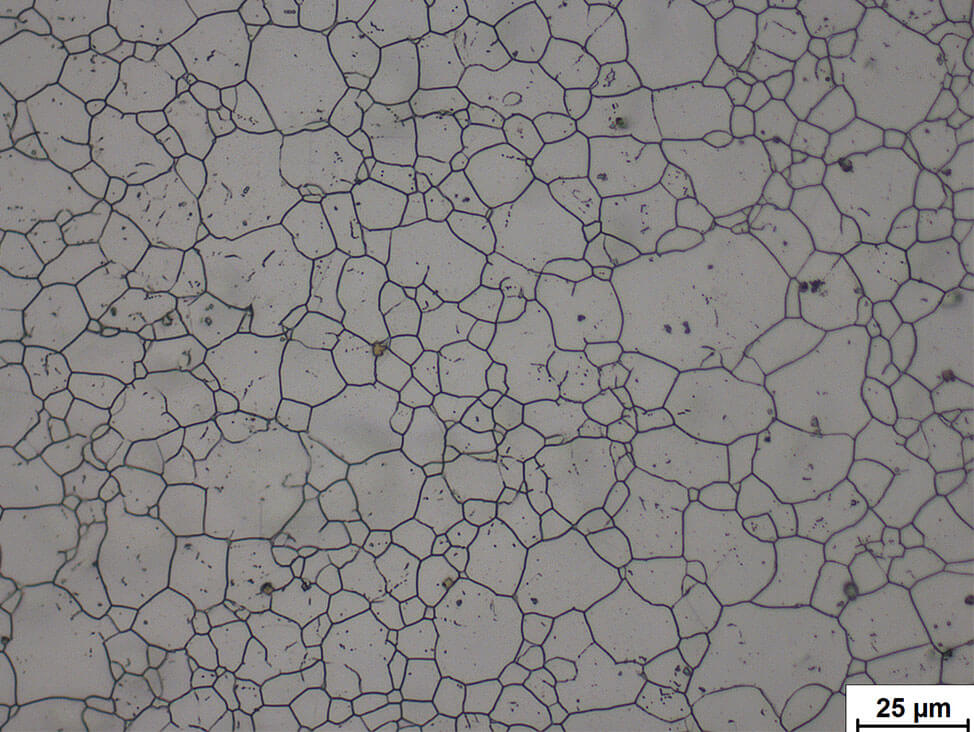
\includegraphics[width=.8\textwidth]{../imgs/fig5} 

}

\caption[Lichtmikroskopische Aufnahme von Austenitischem Stahl.]{Lichtmikroskopische Aufnahme von poliertem und geätztem Austenitischem Stahl, Bild von \emph{Metallographie von Rostfreiem {Stahl}} (\protect\hyperlink{ref-MetallographieRostfreiemStahl}{n.d.}).}\label{fig:baseGrain}
\end{figure}

Um diese Aufnahmen der Schnittbilder zu nutzen, um zu einer quantitativen Beschreibung des Materials zu kommen, wurde traditionell und auch mitunter bis heute eins der vielen ``Linienschnittverfahren'' eingesetzt, wie es zum Beispiel bei Heyn (\protect\hyperlink{ref-heynShortReportsMetallurgical1903}{1903}) beschrieben und als Richtlinienverfahren von der Standardisierungsorganisation ASTM international empfohlen wird (\protect\hyperlink{ref-StandardTestMethods2021}{\emph{Standard {Test Methods} for {Determining Average Grain Size}}, 2021}).
Neben diesem gibt es noch andere Ansätze zum Durchführen der Linienschnitte, alle diese Verfahren haben aber das folgende generelle Verfahren gemeinsam:
Zuerst wird auf eine je nach Verfahren festgelegten Vorgehensweise eine Reihe von Linien in die Aufnahme vom Lichtmikroskop gezeichnet. Diese Linien werden dann genutzt, um die Körner auszuzählen und/oder zu vermessen, die von der Linie geschnitten werden.
Die daraus resultierende Stichprobe an im Werkstück vorhandenen Korngrößen wird abschließend mithilfe einer passenden mathematischen Funktion (z.B. einer log-normalen Verteilungsfunktion) beschrieben, deren Parameter dann als Beschreibung der Kornstruktur genutzt werden.

Neben der verständlichen Ermüdung, die der Bearbeiter bei dieser Methode erfährt, ist die Genauigkeit der Methode grundsätzlich nur approximativ. Daher ist nicht verwunderlich, dass es in diesem Bereich schon Ansätze zur Automatisierung der Materialbeschreibung gibt.
Hier wurde bereits über verschiedene Computervision-Methoden (z.B.: \protect\hyperlink{ref-ananyevCuGdCodoped2014}{Ananyev et al., 2014}; \protect\hyperlink{ref-heilbronnerAutomaticGrainBoundary2000}{Heilbronner, 2000}) und Machine-Learning-Ansätze (z.B.: \protect\hyperlink{ref-decostHighThroughputQuantitative2019}{DeCost et al., 2019}; \protect\hyperlink{ref-dengizGrainBoundaryDetection2005}{Dengiz et al., 2005}) versucht, die Korngrenzen zu extrahieren oder auch die Materialen zu klassifizieren (\protect\hyperlink{ref-abouelattaClassificationCopperAlloys2013}{Abouelatta, 2013}).

Diese Verfahren funktionieren gut zur Segmentation von mit Lichtmikroskopie gewonnenen Kornbildern, die durch Ätzung gut darstellbare Korngrenzen aufweisen.
Da mit dem Fortschritt in der Materialtechnik Körner auf immer kleineren Skalen vorliegen, gewinnt die Anwendung höher auflösender mikroskopischer Verfahren aber zunehmend an Wichtigkeit. Der hier nötige Übergang zur Elektronenmikroskopie stellt die automatische Auswertung der Schnittbilder vor neue Probleme. Zwar können bei ätzbaren Oberflächen die oben genannten automatischen Auswertungsmethoden weiter eingesetzt werden, bei besonders kleinen Körnern führt die Ätzung aber zu einem dermaßen Angriff der Kornstruktur, dass eine Identifikation und Detektion der Grenzen geradezu unmöglich wird.
Stattdessen werden die Körner über ihre je nach kristallographischer Orientierung unterschiedlich starke Beugung der Elektronen im Rückstreubild in unterschiedlichen Graustufen dargestellt. Diese Graustufenbilder machen das Identifizieren der Korngrenzen ungemein schwieriger. Beispiele für solche Aufnahmen sind in Abbildung \ref{fig:electroGrain} zu sehen.





\begin{figure}

{\centering 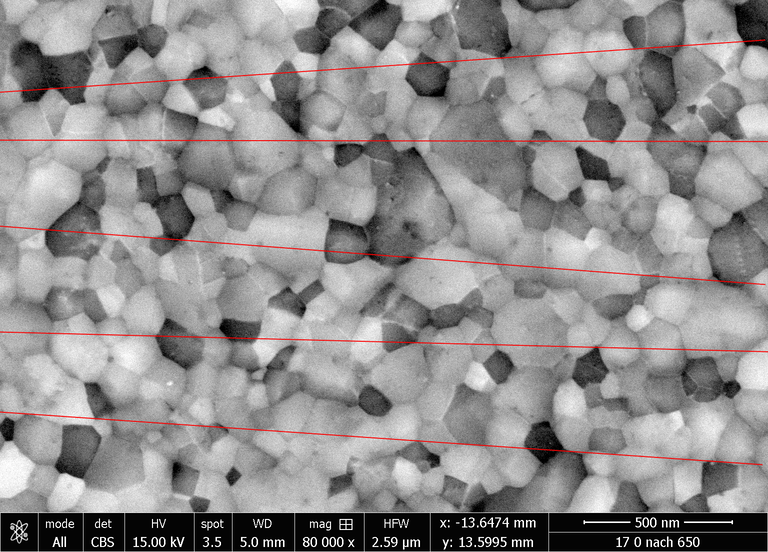
\includegraphics[width=.45\textwidth]{../imgs/out1} 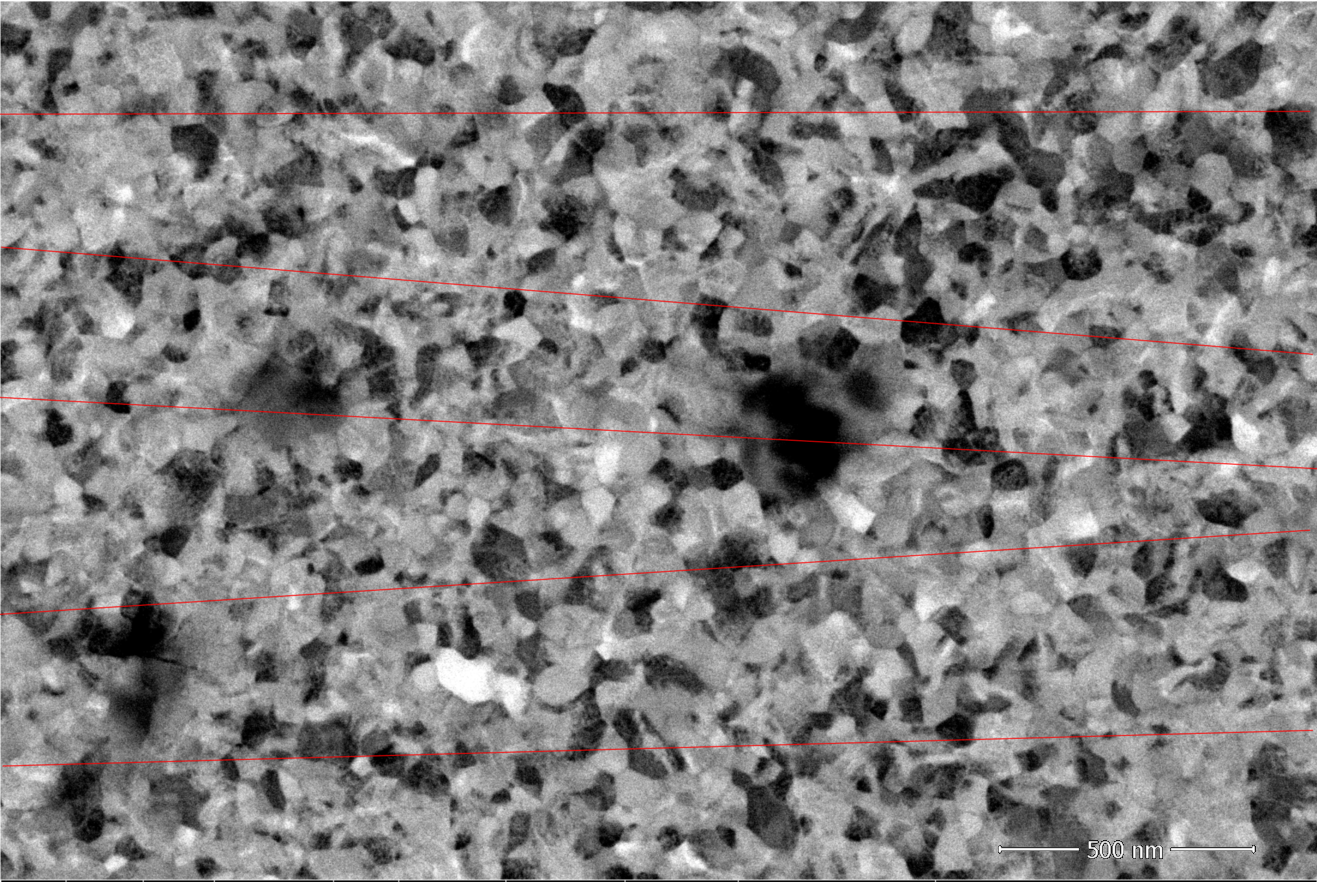
\includegraphics[width=.45\textwidth]{../imgs/out2} 

}

\caption[Elektronenmikroskopische Aufnahmen von Werkstücken.]{Elektronenmikroskopische Aufnahmen von Werkstücken. In rot sind die Linien eingezeichnet, die zur Bestimmung der Kornverteilung mit Hilfe eines Linienschnittverfahrens eingesetzt wurden. Das Werkstück links weist wenig Artefakte und klar zu erkennende Kornflächen auf. Rechts ist ein Werkstück abgebildet, dessen Körner weniger deutlich zu erkennen sind, das Gradienten von Grautönen in einem Korn aufweist und dessen Aufnahme deutliche Bildartefakte produziert hat.}\label{fig:electroGrain}
\end{figure}

Zusätzlich stören Kristalldefekte, Oberflächenartefakte und Spannungen im Material die Auswertung, da sie zu überlagernden Kontrastartefakten führen (Abbildung \ref{fig:electroGrain} rechts).
Mit Training sind menschliche Bearbeiter zwar weiter in der Lage, Körner und ihre Grenzen zu detektieren und mit Linienschnittverfahren auszuwerten, bestehende Ansätze zur automatischen Detektion von Korngrenzen scheitern aber.

Im Bereich der Mineral-Korn-Erkennung wurden aber bereits erfolgreich vielversprechende Ansätze berichtet (\protect\hyperlink{ref-latifDeepLearningBasedAutomaticMineral2022}{Latif et al., 2022}; \protect\hyperlink{ref-maitreMineralGrainsRecognition2019}{Maitre et al., 2019}). Diese neuen Ansätze haben gemeinsam, dass sie statt Korngrenzen deren Flächen auszumachen versuchen. Dabei werden Methoden der \emph{Superpixel Segmentation} eingesetzt, bei denen versucht wird, ein Bild in semantisch ähnliche Gruppen von Pixeln zu segmentieren. Das Aufteilen eines Bildes in Superpixel ist ein reduzieren der Bildkomplexität für folgende Analyseschritte (\protect\hyperlink{ref-wangSuperpixelSegmentationBenchmark2017}{Wang et al., 2017}). Eine Anwendung von Superpixel-basierten Ansätzen zur Segmentation von mikroskopischen Aufnahmen von Metallstrukturen sind entweder zu hochauflösend (\protect\hyperlink{ref-akersRapidFlexibleSegmentation2021}{Akers et al., 2021}), zu niedrig auflösend (\protect\hyperlink{ref-kimUnsupervisedMicrostructureSegmentation2020}{Kim et al., 2020}) oder auf andere Arten von Mineral bezogen (\protect\hyperlink{ref-decostHighThroughputQuantitative2019}{DeCost et al., 2019}; \protect\hyperlink{ref-latifDeepLearningBasedAutomaticMineral2022}{Latif et al., 2022}) oder nur auf Teile der Aufnahme bezogen (\protect\hyperlink{ref-liMetallographicImageSegmentation2020}{li et al., 2020}).

Da die Vorbereitung und das spezifische ausgewertete Material stark die Art und Qualität der Bilder beeinflusst, lassen sich diese Ergebnisse nicht direkt auf Aufnahmen von dünnen Schichten übertragen - die Ansätze scheinen aber vielversprechend. Die Auswertung von Größe und Orientierung möglichst aller Körner über die gesamte elektronenmikroskopische Aufnahme dünner Schichten ist jedoch bisher noch von keinem dieser Ansätze gelöst.

Die vorliegende Masterarbeit soll an diesem Punkt ansetzen und versuchen, auf Basis von Superpixel-Verfahren möglichst alle Körner in einer elektronenmikroskopisch aufgenommenen Gitterstruktur zu erkennen und diese zu vermessen.

\hypertarget{zielsetzung}{%
\section{Zielsetzung}\label{zielsetzung}}

Das Ziel dieser Abschlussarbeit ist die Entwicklung eines Tools, das mindestens die Auswertung von Kornbildern unterstützt und im besten Fall diese übernimmt.
Als erster Schritt ist dafür eine Implementierung mit grafischer Oberfläche nötig, die das Einlesen und Verarbeiten von elektronenmikroskopischen Aufnahmen mit dahinter stehendem Datenmodell unterstützt.
Dabei soll die Verarbeitung sowohl aus dem Vorverarbeiten, als auch der Kornerkennung und -vermessung bestehen.
Der Nutzen des Tools soll durch Angehörige des Instituts getestet und dessen Nutzbarkeit überprüft werden. Die bei dieser Überprüfung entstehenden Wünsche an Verbesserungen und Anpassungen des Programms sollen so weit wie möglich umgesetzt werden.

Im zweiten Schritt soll auf dem Datenmodell aufbauend versucht werden, mit Hilfe von Superpixel- und ML-Modellen die Auswertung durch Einstellungs-Empfehlungen zu unterstützen oder im besten Falle zu übernehmen.

\hypertarget{unternehmensvorstellung}{%
\section{Unternehmensvorstellung}\label{unternehmensvorstellung}}

Die Arbeit wird in enger Abstimmung mit dem Institut für Materialphysik der Georg-August-Universität Göttingen umgesetzt und basiert auf dort aufgenommenen und per Linienschnitt ausgewerteten Kornbildern.
Die Georg-August-Universität Göttingen wurde 1734 gegründet und zählt mit ihren 29.167 Studierenden im WiSe 21/22 (\protect\hyperlink{ref-offentlichkeitsarbeitStudiumUndLehre}{Öffentlichkeitsarbeit, n.d.-b}) und den 5.165 Beschäftigten im Jahr 2021 (\protect\hyperlink{ref-offentlichkeitsarbeitPersonalGeorgAugustUniversitatGottingen}{Öffentlichkeitsarbeit, n.d.-a}) zu den größten Hochschulen Deutschlands. Am Lehrstuhl für Materialphysik wird regelmäßig das Verhalten von Materialien in dünnen Schichten untersucht, deren Oberflächen dazu elektronenmikroskopisch aufgenommen und händisch per Linienschnitt ausgewertet werden.

\hypertarget{aufbau-der-arbeit}{%
\section{Aufbau der Arbeit}\label{aufbau-der-arbeit}}

Im Folgenden wird zuerst auf die Grundlagen der verwendeten Filter- und Auswertungsmethoden und deren Funktionsprinzipien eingegangen.
Im Darauf folgenden Kapitel wird die das Anforderungsprofil der Anwendung formuliert, gefolgt durch eine Beschreibung der Entwicklung des Tools und der Ansätze zur Unterstützung auf Basis maschinellen Lernens.
Der Nutzen des Tools wird im vorletzten Kapitel evaluiert, wonach Abschließend eine Schlussbetrachtung inklusive weiterer zu verfolgender Ansätze folgt.

\hypertarget{grundlagen}{%
\chapter{Grundlagen}\label{grundlagen}}

Dieses Kapitel beschäftigt sich zuerst mit den zur Bildvorbereitung betrachteten und verwendeten Algorithmen. Darauf folgt eine Beschreibung der getesteten Ansätze zur Flächen-Gruppierung um dann dazu überzugehen, die Implementation des Körner-Tools zu beschreiben.
Im Anschluss werden die verwendeten Ansätze zur Stapelverarbeitung der Bilder beschrieben.

\hypertarget{bildvorverarbeitung}{%
\section{Bildvorverarbeitung}\label{bildvorverarbeitung}}

Im folgenden werden die einzusetzenden Vorverarbeitungsalgorithmen beschrieben. Da das Augenmerk dieser Arbeit insbesondere auf der Erkennung von Körnern und weniger auf dem Preprocessing liegen soll, wurde sich hier vor allem auf bereits in der Kornvermessung eingesetzte Algorithmen gestützt.
Alle diese Vorverarbeitungs-Schritte verfolgen zwei Ziele:
Zum Einen soll versucht werden, die Bildartefakte so gut wie möglich zu entfernen, zum Anderen sollen die Grautöne innerhalb eines Korns so sehr angeglichen werden, wie möglich.
Die Reihenfolge der Algorithmen ist außerdem von entscheidender Bedeutung, ein Histogramm-Equalizer führt nach Anwendung eines Gauss-Filters zu einem deutlich anderen Effekt als davor. Auf diesen Punkt wird aber in der Beschreibung der Implementation noch umfangreicher eingegangen.

\hypertarget{gauss-filter}{%
\subsection{Gauss-Filter}\label{gauss-filter}}

Gauss-Filter sind häufig in Anwendungsbereichen mit stark multivariaten Untersuchungsgegenständen zu beobachten, so zum Beispiel in EEG- und fMRT-Analysen (\protect\hyperlink{ref-harishvijeyAutomatedTechniqueEEG2022}{Harishvijey \& Benadict Raja, 2022}; \protect\hyperlink{ref-winkDenoisingFunctionalMR2004}{Wink \& Roerdink, 2004}), in Zeitreihenanalysen (\protect\hyperlink{ref-kitagawaTwofilterFormulaSmoothing1994}{Kitagawa, 1994}) und nicht zuletzt weit verbreitet in der Bildverarbeitung (\protect\hyperlink{ref-basuGaussianbasedEdgedetectionMethodsa2002}{Basu, 2002}).

Bei diesem Verfahren wird das Bild mit Hilfe einer zweidimensionalen Gauss-Verteilung gefaltet, wodurch jedes Pixel durch die gewichtete Summe der umherliegenden Pixel ersetzt wird. Die dabei eingesetzte zweidimensionale Dichte-Funktion wird häufig als der \emph{Kernel} bezeichnet. In Abb. \ref{fig:gaussFilter} ist beispielhaft das Ergebnis eines Gauss-Filters zu sehen, in der dessen primäre Funktion deutlich wird.
Dieser auch als Glättungs-Filter bezeichnete Vorverarbeitungs-Algorithmus wird mit dem Ziel eingesetzt, einzelne Pixel mit im Vergleich mit dem direkten Umfeld extremen Werte anzugleichen und so Bildartefakte zu entfernen.





\begin{figure}

{\centering 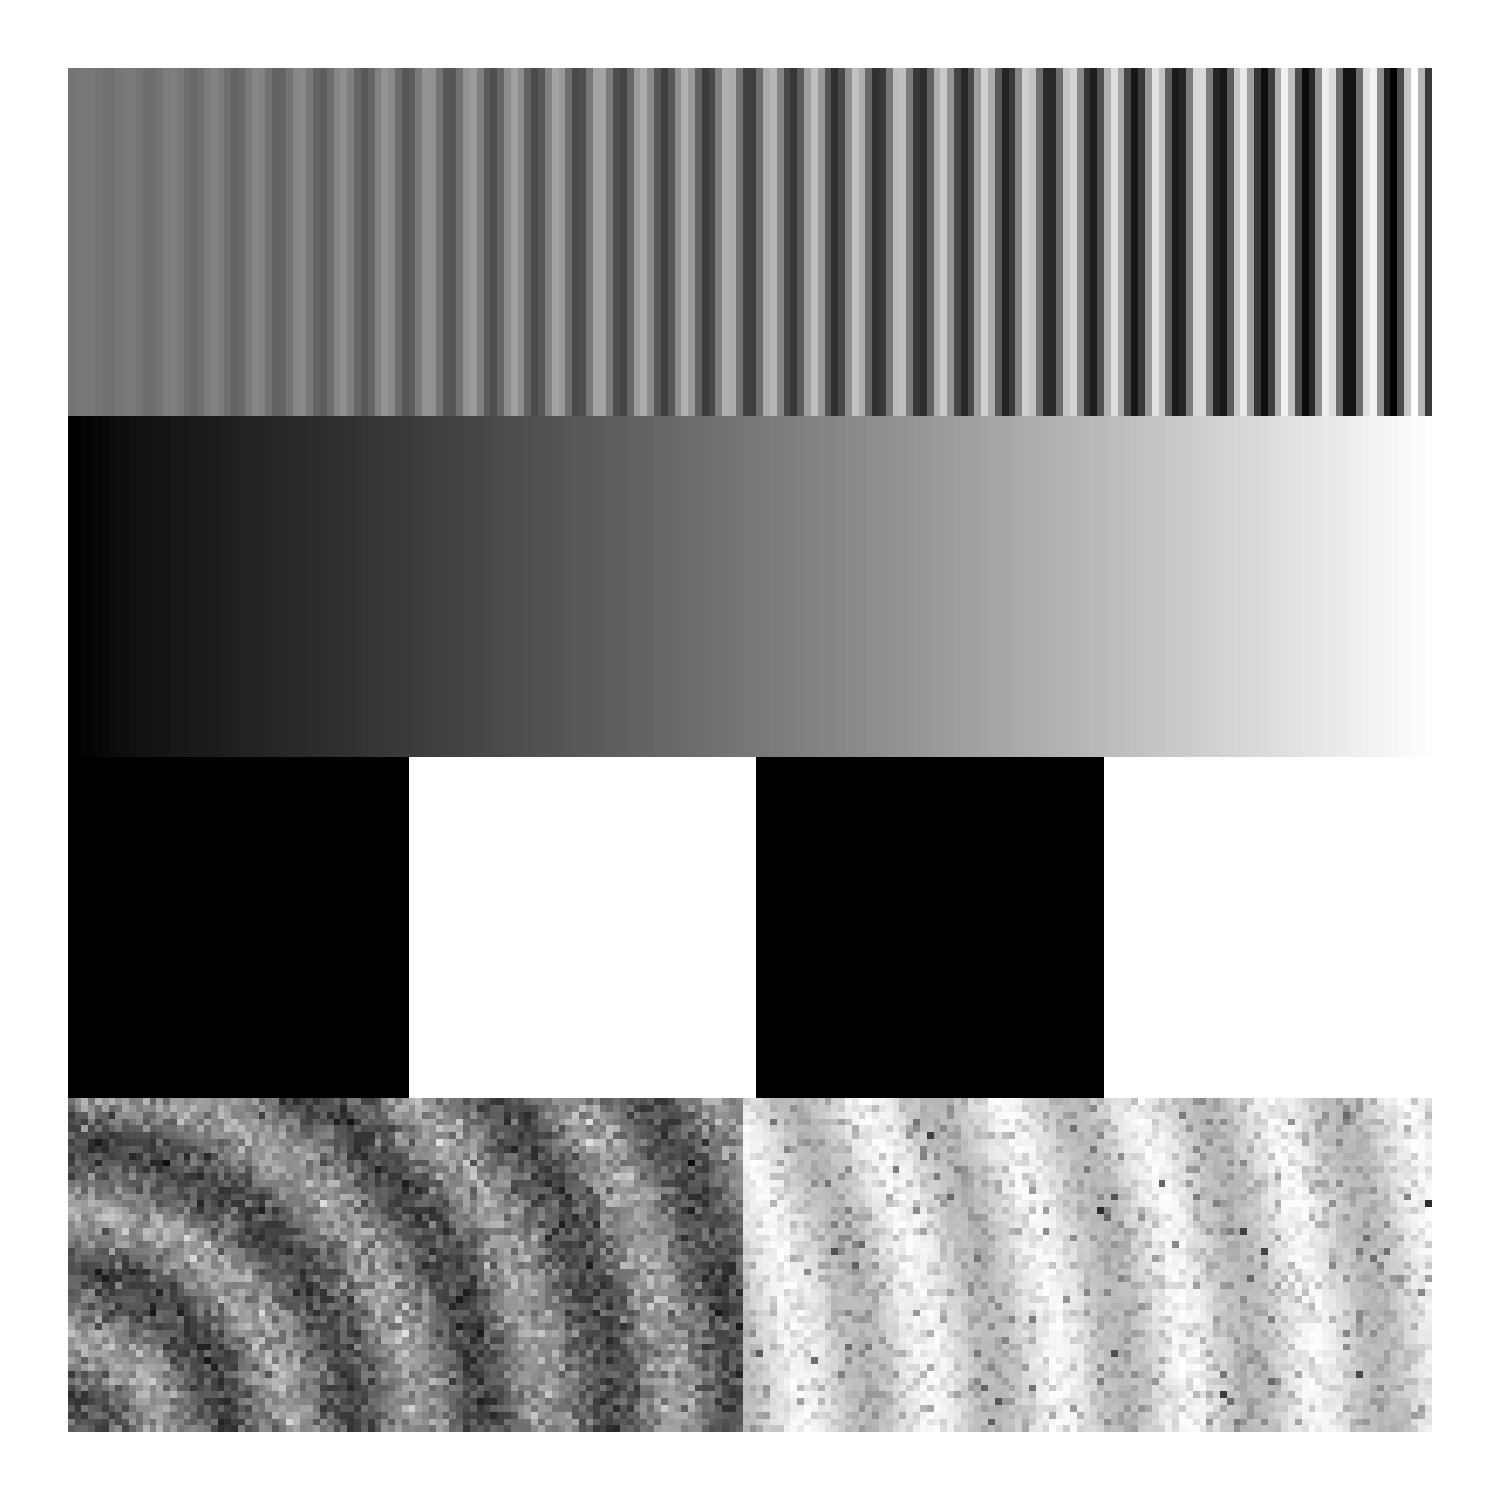
\includegraphics[width=.32\textwidth]{../imgs/geometric} 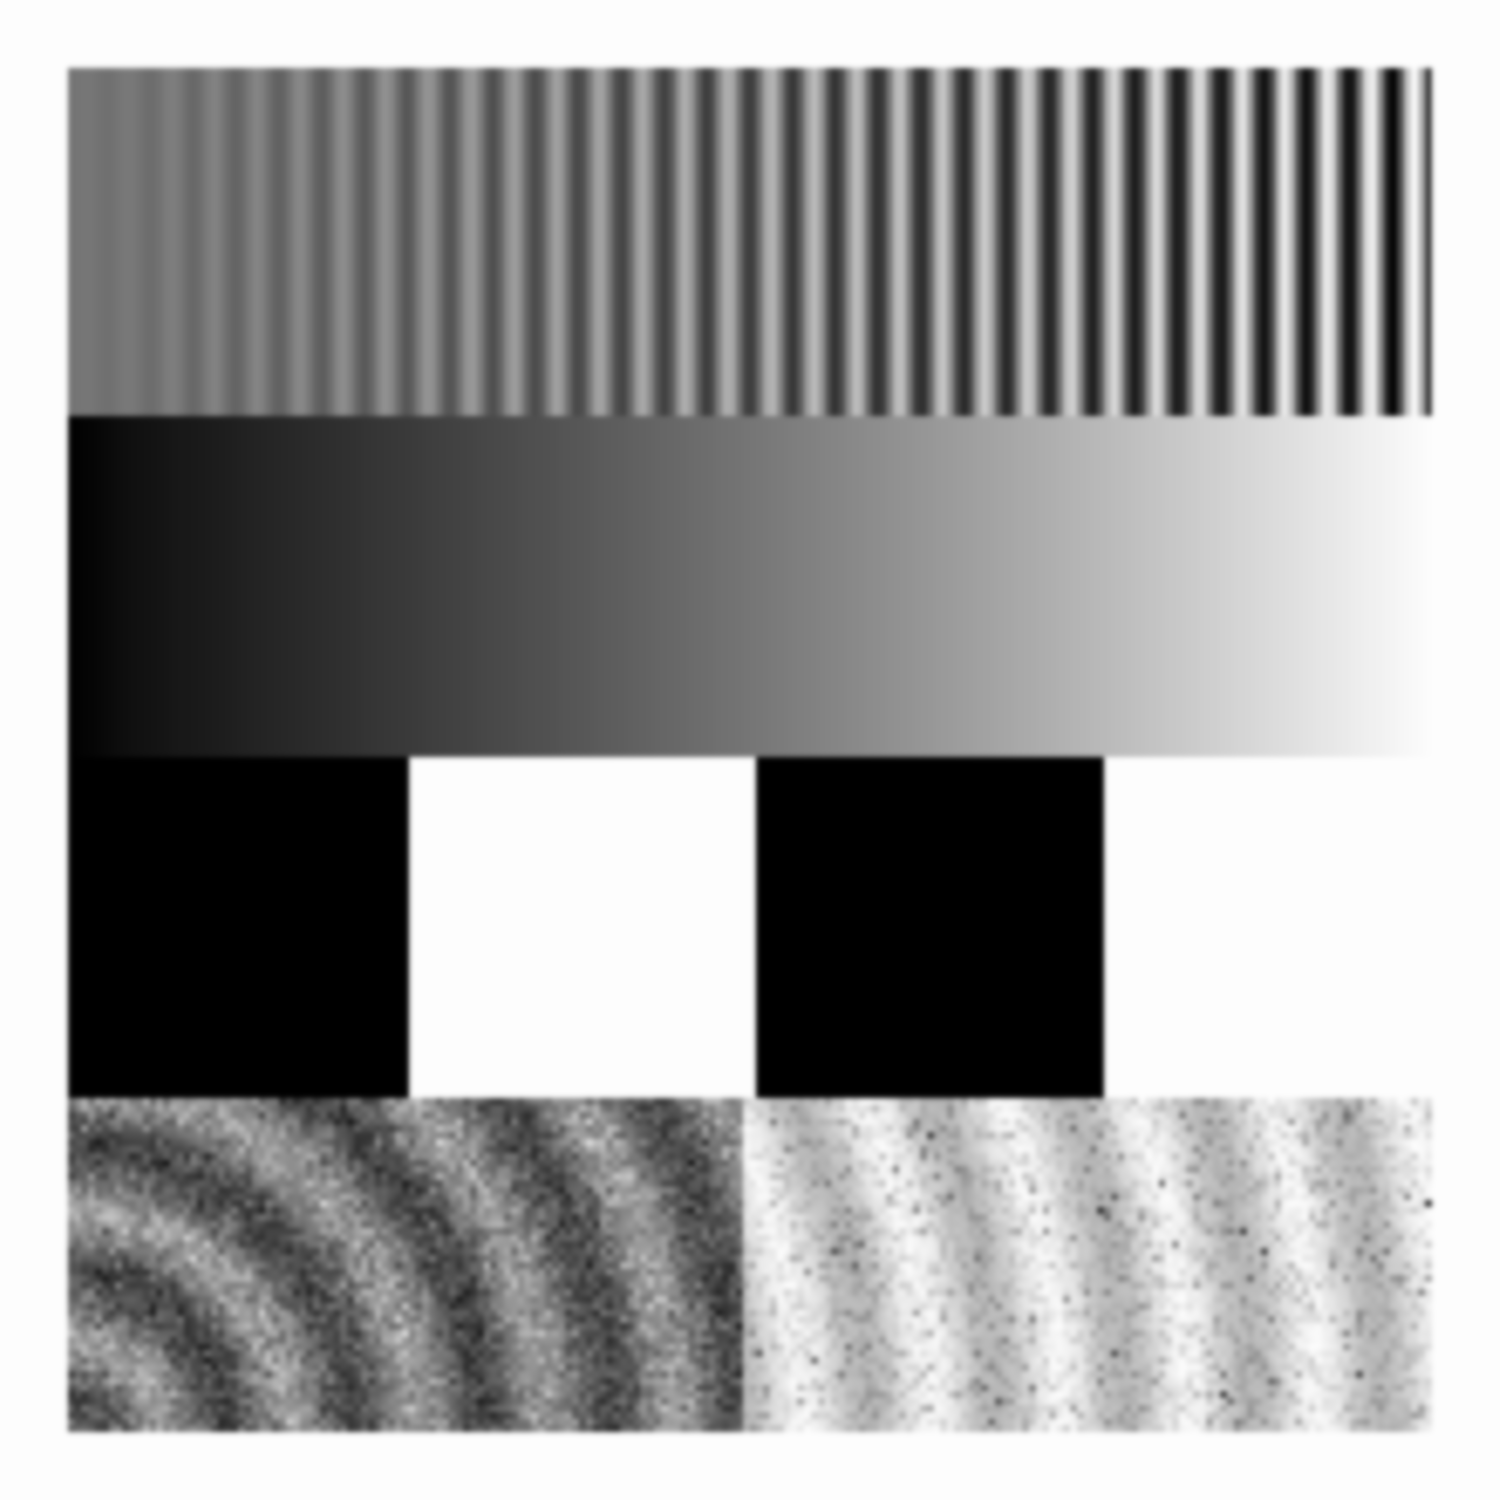
\includegraphics[width=.32\textwidth]{../imgs/gauss15} 
\includegraphics[width=.32\textwidth]{../imgs/gauss150} 

}

\caption[Beispiel eines Gauss-Filters.]{Beispiel eines Gauss-Filters. Links ist das Bild vor dem Filtern, in der Mitte nach dem Filtern mit einem Gausskernel mit Durchmesser von 15 Pixeln (1\% der Bildkantenlänge) und rechts einem mit Durchmesser von 151 Pixeln (\textasciitilde10\% der Kantenlänge) zu sehen.}\label{fig:gaussFilter}
\end{figure}

\hypertarget{histogramm-equalizer}{%
\subsection{Histogramm-Equalizer}\label{histogramm-equalizer}}

Ein Histogramm-Equalizer gleicht die Helligkeitswerte eines Bilds so an, dass deren kumulative Häufigkeitsverteilung linear ansteigt (\protect\hyperlink{ref-princePartIVPreprocessing2012}{Prince, 2012}). Je nach Bild kann es also passieren, dass Teile der Helligkeitswert-Verteilung gestreckt, andere Teile gestaucht werden.
Diese nicht-lineare Transformation führt dazu, dass bei ungleichen Helligkeitsverteilung, wie zum Beispiel im Falle eines Bildes mit vielen ähnlichen Grautönen, vorher kleine Unterschiede deutlicher Akzentuiert werden, während stark unterschiedliche Helligkeitswerte angenähert werden können.

In Abb. \ref{fig:histEqual} ist der Effekt des Histogramm-Equalizers beispielhaft dargestellt.





\begin{figure}

{\centering 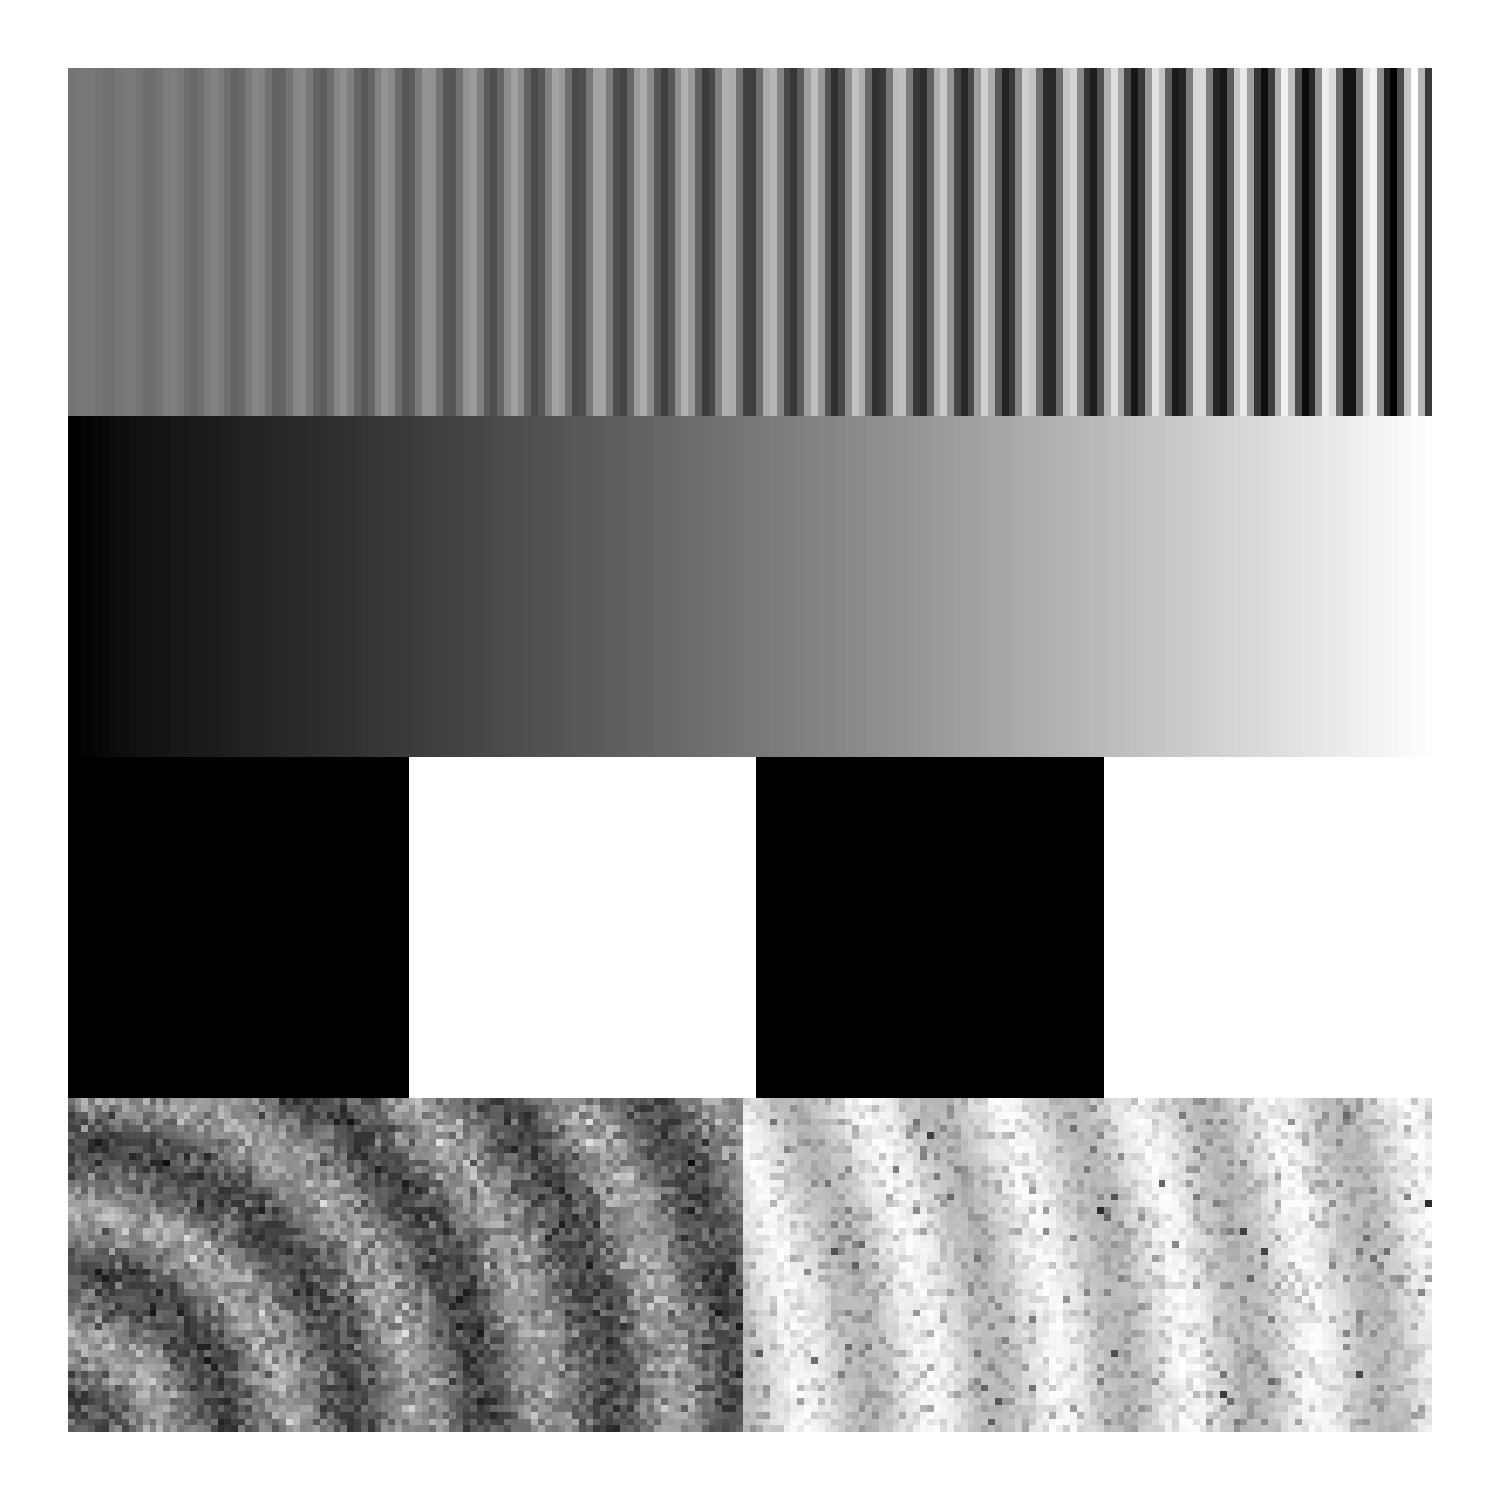
\includegraphics[width=.48\textwidth]{../imgs/geometric} 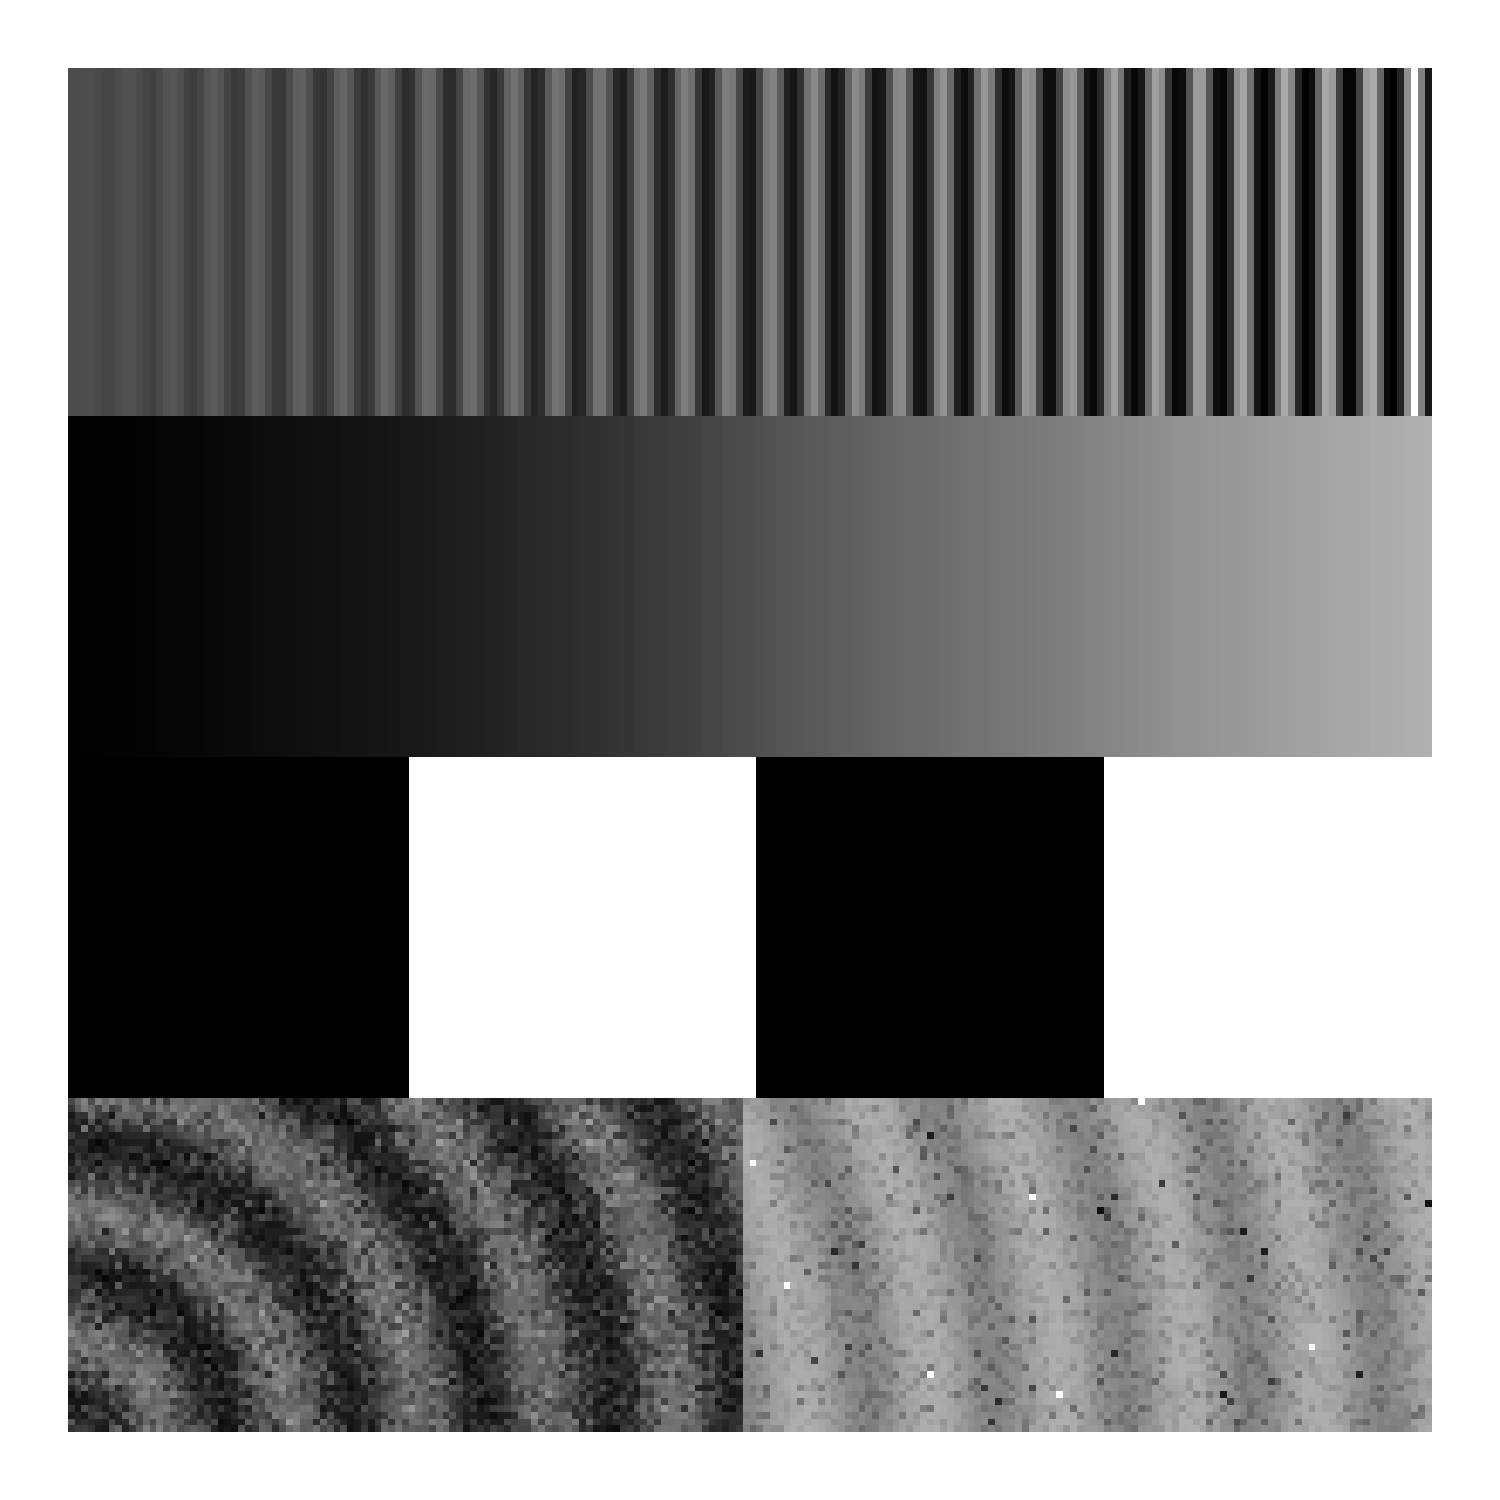
\includegraphics[width=.48\textwidth]{../imgs/hist_equal} 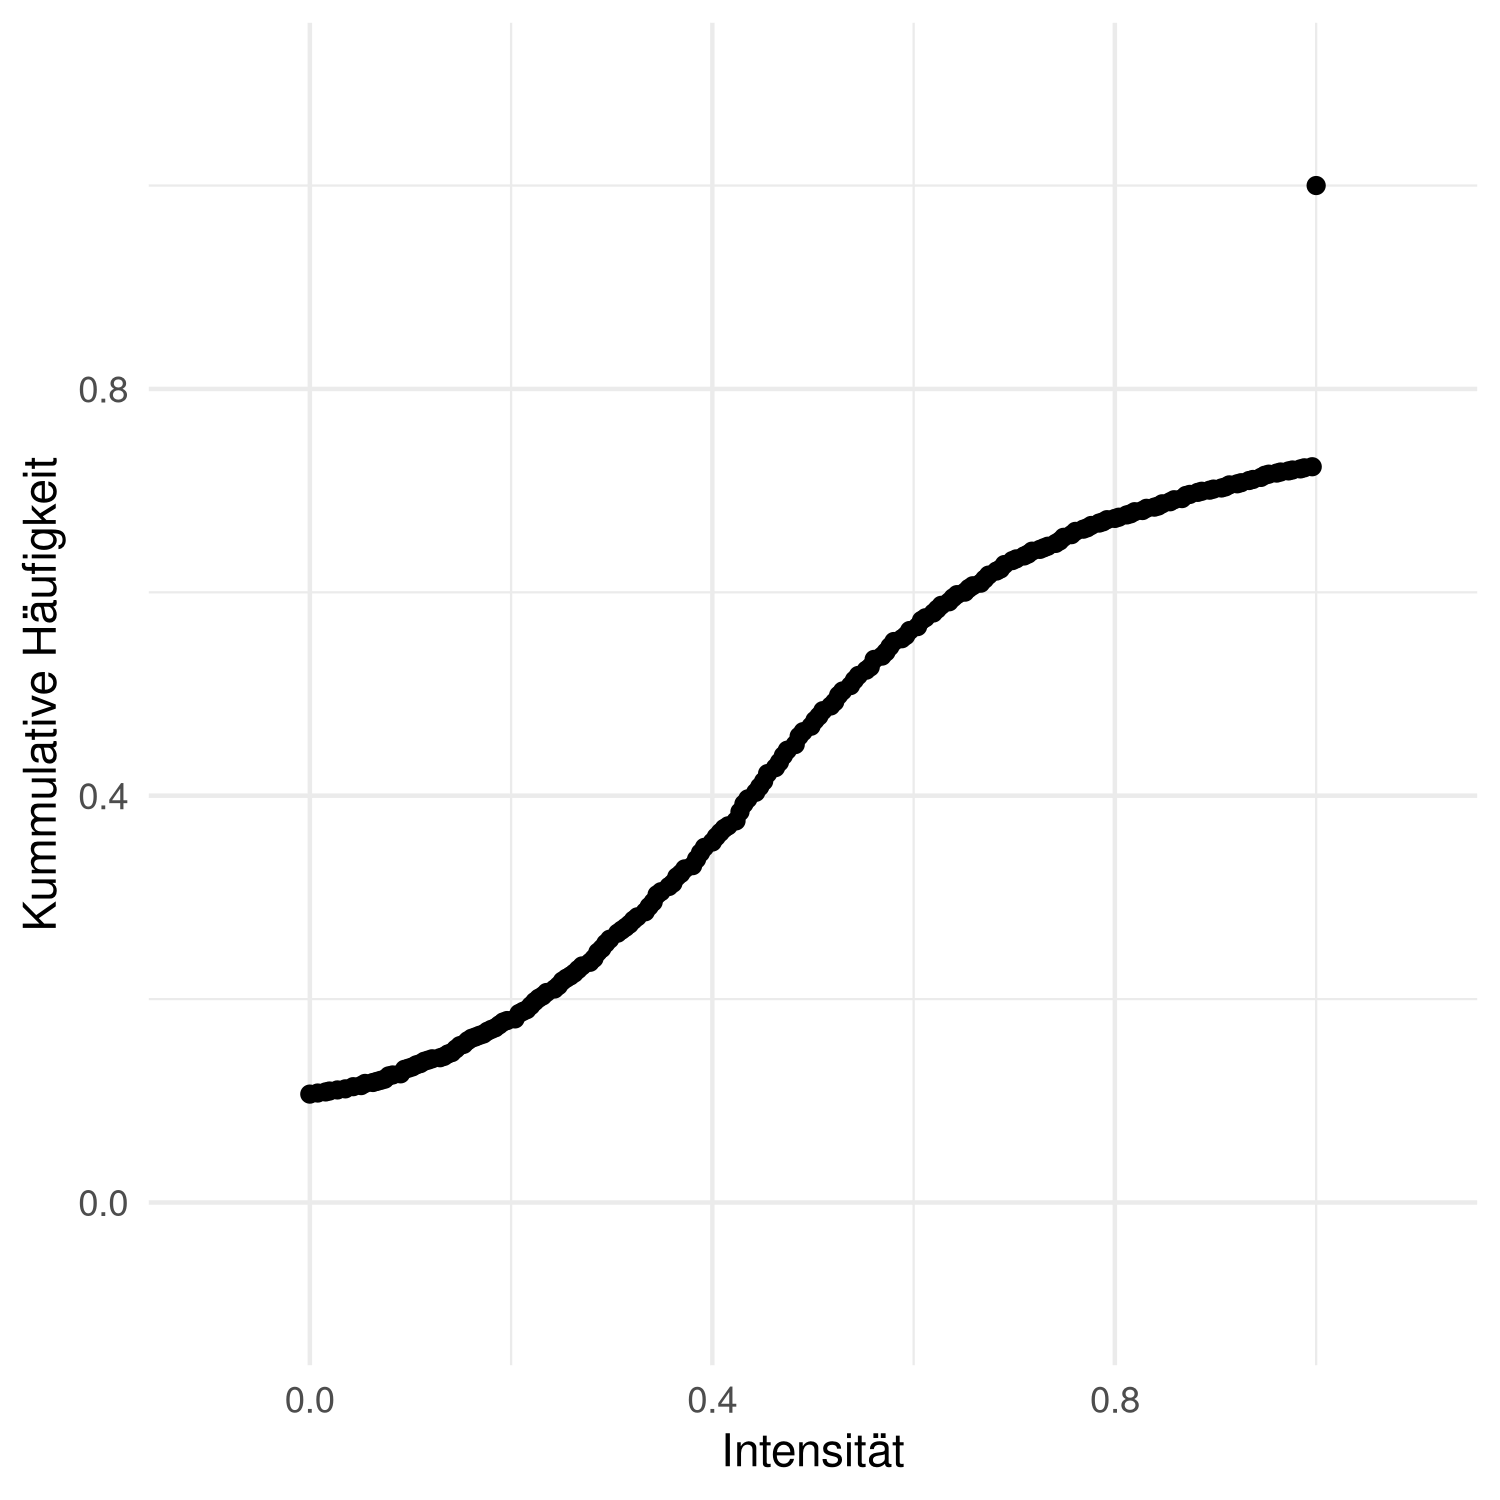
\includegraphics[width=.48\textwidth]{../imgs/hist_kum1} 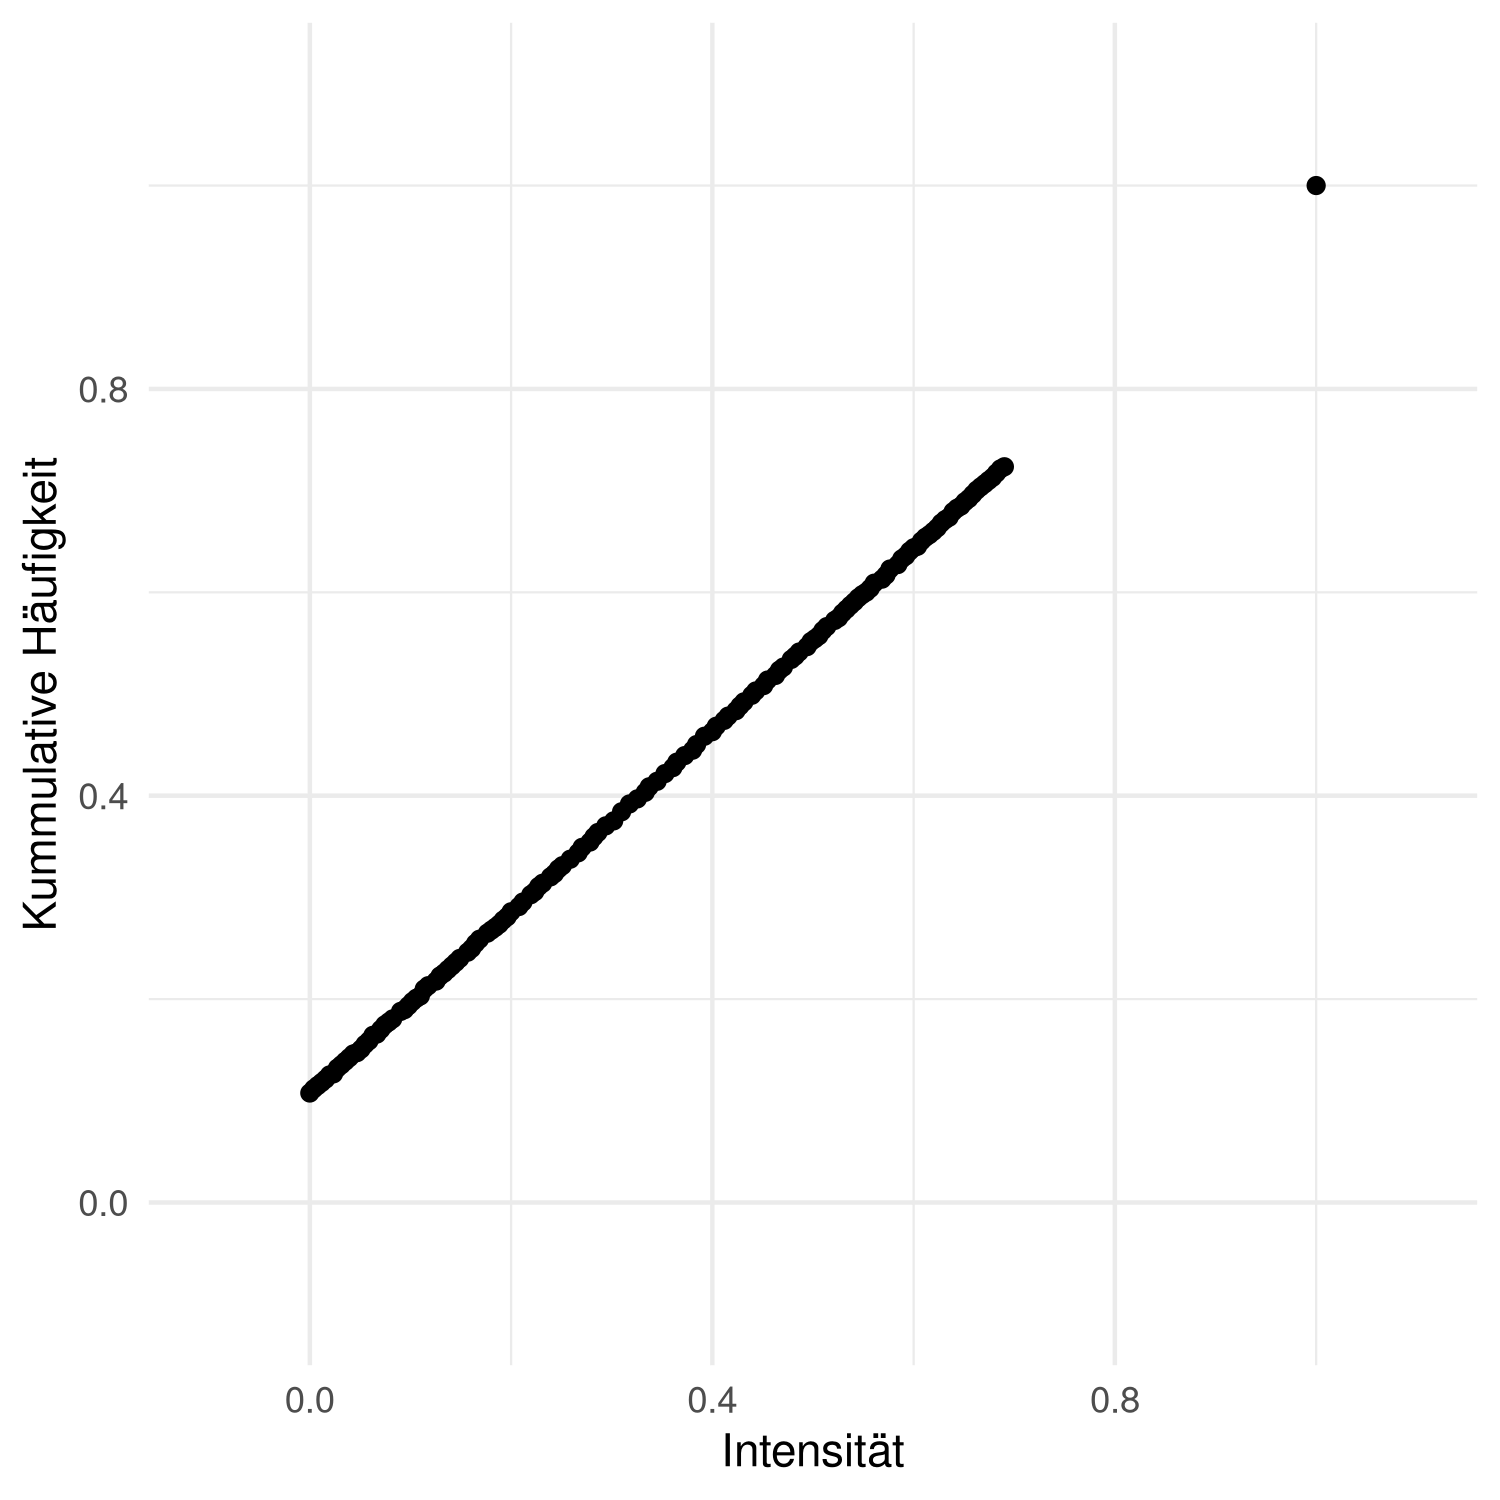
\includegraphics[width=.48\textwidth]{../imgs/hist_kum2} 

}

\caption[Beispiel für die Anwendung eines Histogramm-Equalizers.]{Beispiel für die Anwendung eines Histogramm-Equalizers. Links ist das Bild vor, rechts nach der Anpassung der Helligkeitsverteilung zu sehen. Der Farbverlauf wurde verdunkelt, genau wie die erste, auf dem Cosinus basierenden Zeile mit Ausnahme einer weißen Spalte. Unten sind die Helligkeitsverteilungen abgebildet, die Linearisierung ist deutlich zu erkennen.}\label{fig:histEqual}
\end{figure}

\hypertarget{non-local-mean-denoiser}{%
\subsection{Non-Local-Mean-Denoiser}\label{non-local-mean-denoiser}}

Ein Non-Local-Mean Denoiser versucht wie der Name schon sagt, Bildrauschen durch das Bilden nicht lokaler Mittelwerte zu bilden. Dazu wird in einem angegebenen Suchfenster für alle ähnlich grauen Pixel der Mittelwerte der Grauwerte gesetzt. Die Pixel müssen dabei explizit nicht lokal nebeneinander liegen, sondern nur einen ählichen Grauwert aufweisen (\protect\hyperlink{ref-buadesNonLocalMeansDenoising2011}{Buades et al., 2011}).

Der Filter wird dabei über eine Filter-Stärke, die Größe des Suchfensters und die Größe des ``Templates'', also der Menge als gleich gezählter Pixel bestimmt.

In Abb. \ref{fig:nlMeans} ist der Effekt des Denoisers zu sehen, das Bildrauschen im Unteren Viertel wird deutlich reduziert, auch wenn das Muster dadurch leicht undeutlich wird. Der Denoiser stößt jedoch an seine Grenzen bei der Entfernung nicht-normalen Rauschens, wie zum Beispiel in der rechten Hälfte der letzten Zeile zu sehen ist. Dort wurde im Gegensatz zur linken Hälfte kein normalverteiltes, sonder F-verteiltes Rauschen auf das Bild addiert.





\begin{figure}

{\centering 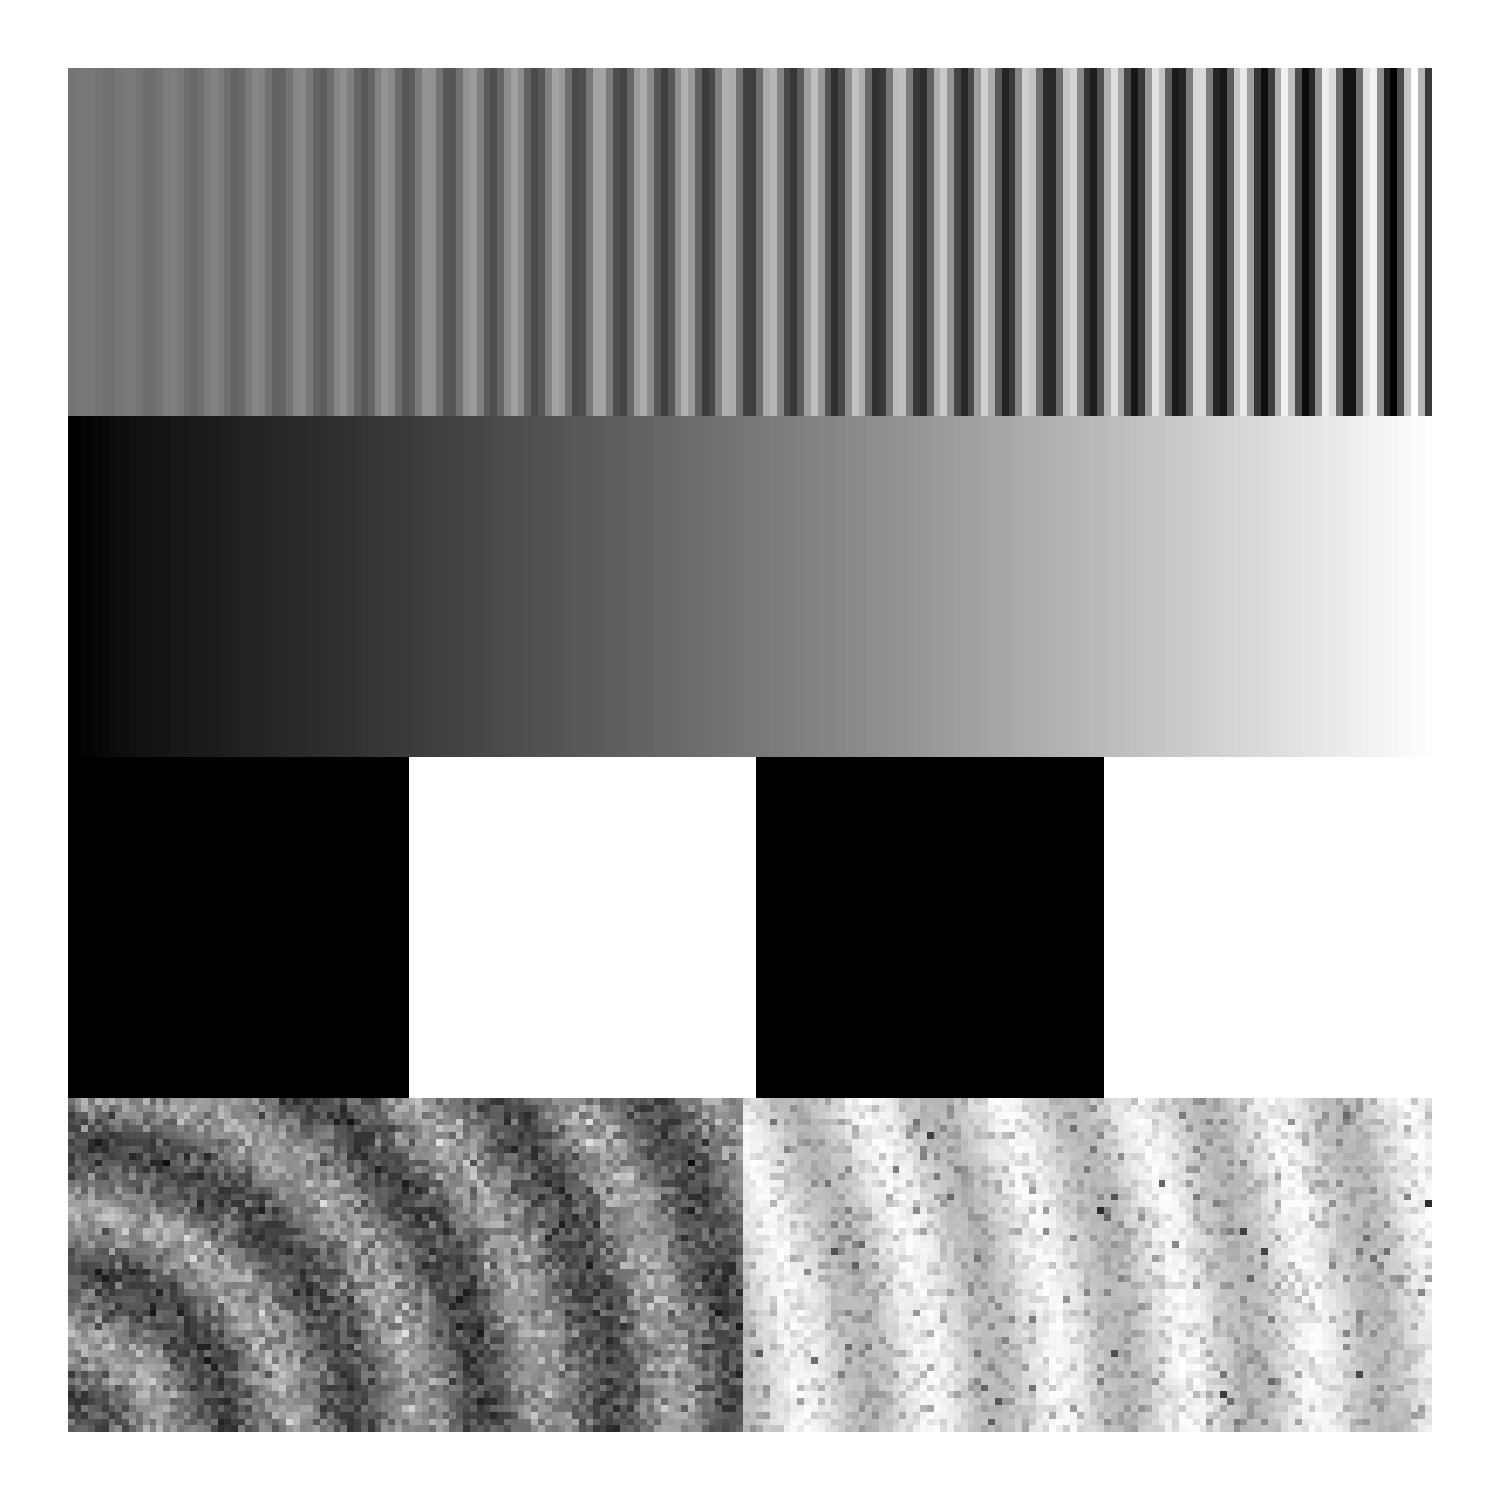
\includegraphics[width=0.48\textwidth]{../imgs/geometric} 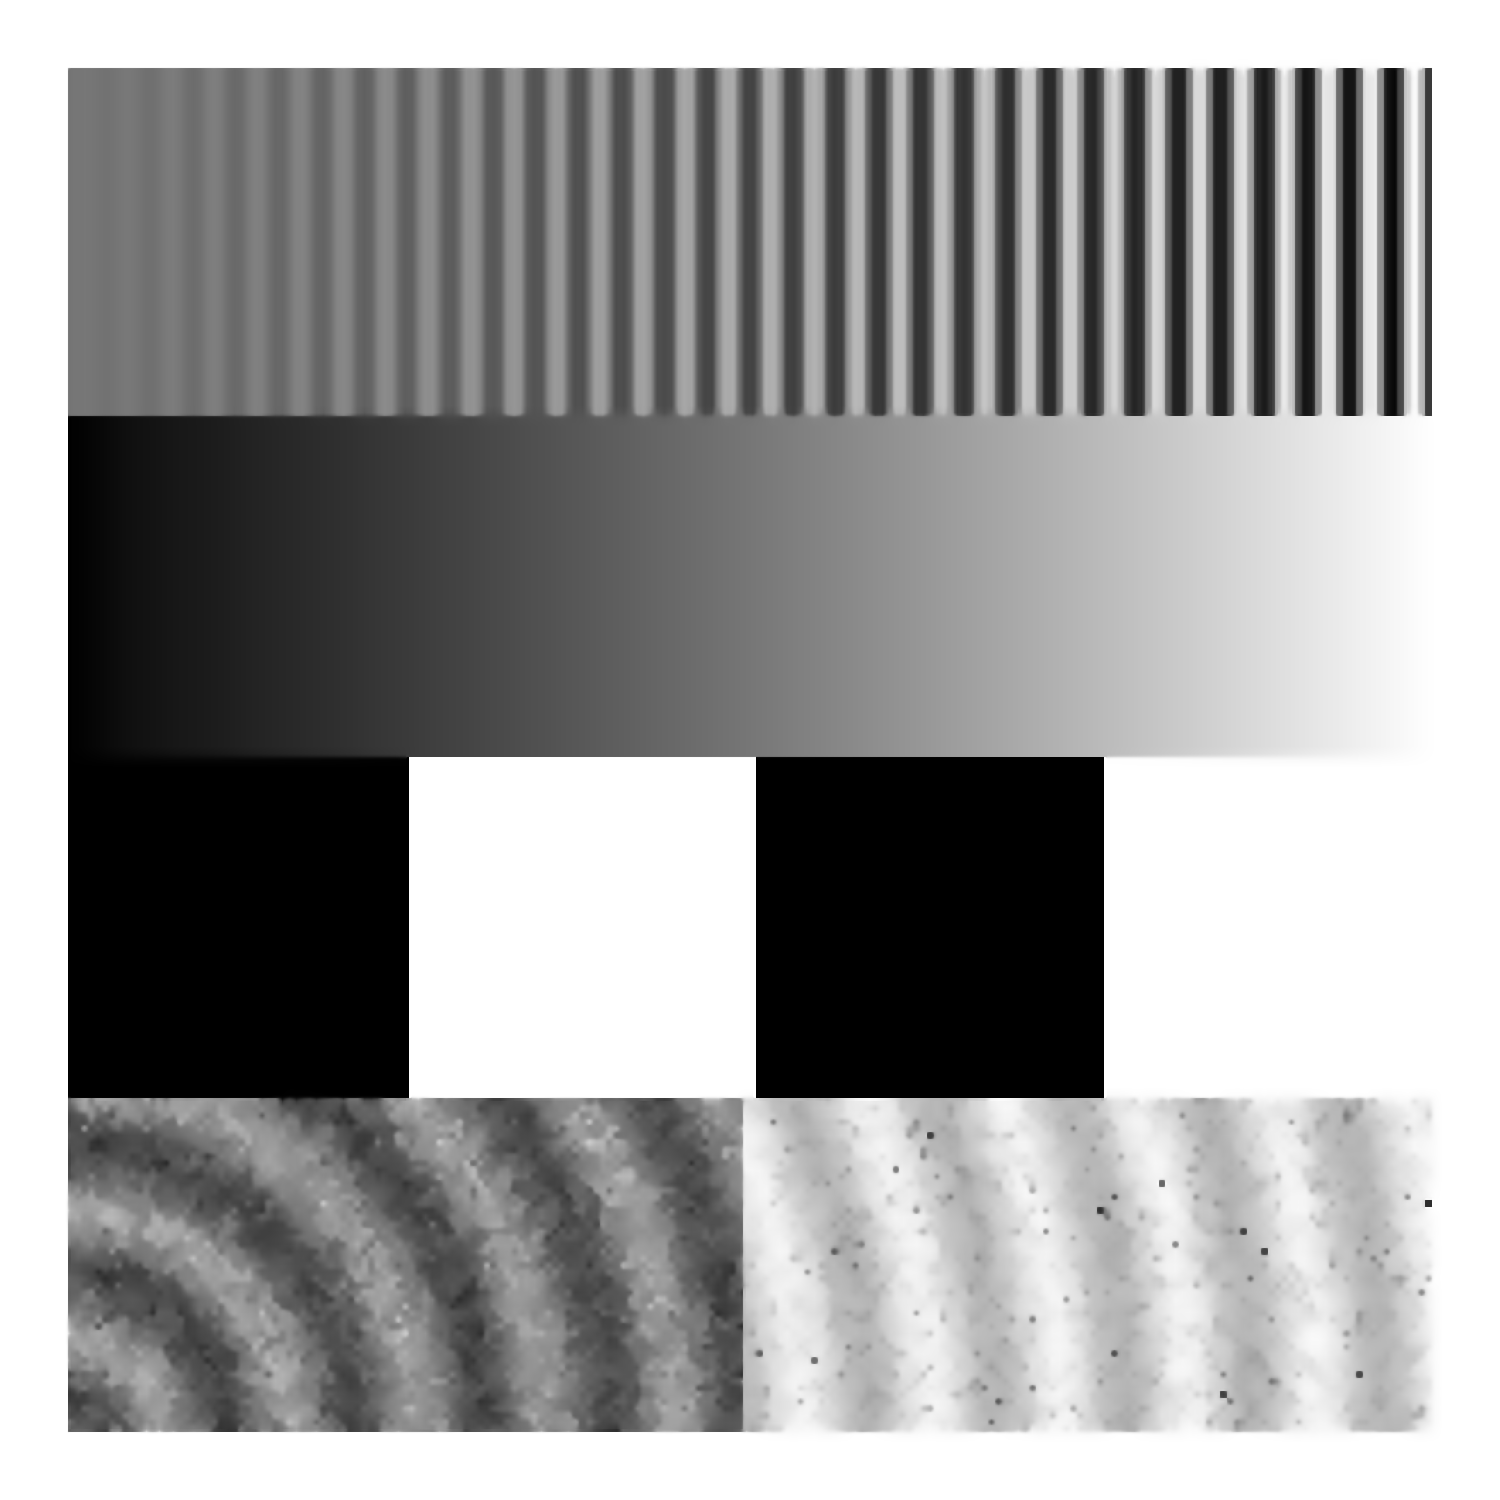
\includegraphics[width=0.48\textwidth]{../imgs/nlMean_30_7_21} 

}

\caption[Beispiel für die Anwedung eines Non-Local\_Mean Denoisers.]{Beispiel für die Anwedung eines Non-Local\_Mean Denoisers. Links ist das Bild, rechts nach dem Denoising mit einer Template-Größe von 7, einem Suchfenster von 21 zu sehen, der Filter wurde ziemlich stark gewichtet um den Einfluss deutlich zu machen. Das Rauschen wurde zwar reduziert, die konzentrischen Kreise aber auch unschärfer.}\label{fig:nlMeans}
\end{figure}

\hypertarget{savitzky-golay-filter}{%
\subsection{Savitzky-Golay-Filter}\label{savitzky-golay-filter}}

Ein Savitzky-Golay-Filter wird in allen Bereichen der Signalverarbeitung zur Signalglättung eingesetzt. Dabei wird in einem Fenster mit vorgegebener Größe der Signalreihe Stück für Stück ein festgelegte Polynome Regression durchgeführt. Das Mittel der Vorhersagen über die Datenreihe wird dann zurückgegeben. Je nach Größe des Fensters und der Höhe des Polynoms wird dadurch unterschiedlich stark geglättet.

In Abb. \ref{fig:savgol} ist der Effekt des eines horizontalen und vertikalen Savitzky-Golay-Filter mit jeweils einer Fenstergröße von 51 Pixeln, und einem Polygon der 1., 5. und 11. Ordnung beispielhaft dargestellt. Wie zu sehen ist, schlägt sich der Filter bei niedrigen Polynomen eher als Unschärfe nieder, je höher die Polynome sind desto mehr Varianz im Signal wird nicht entfernt.





\begin{figure}

{\centering 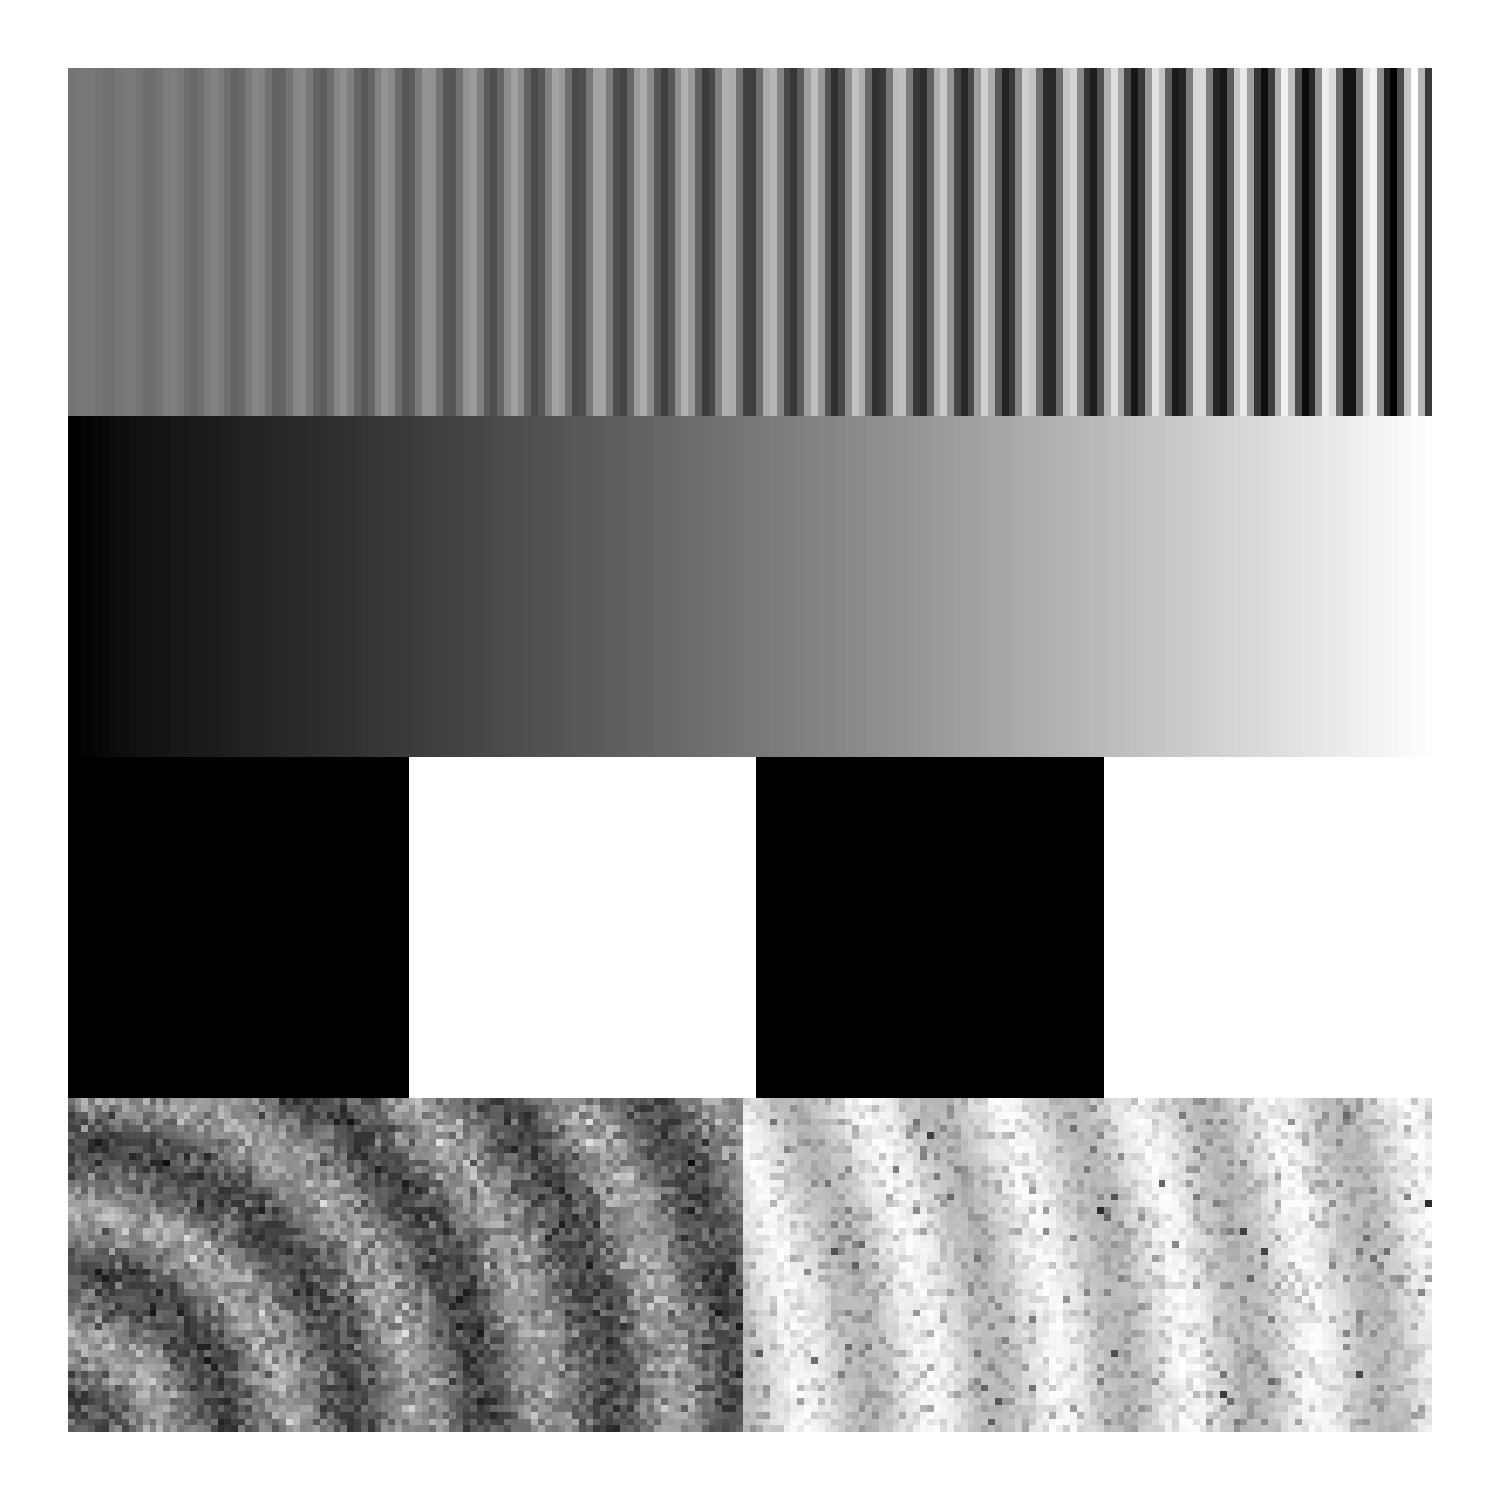
\includegraphics[width=.24\textwidth]{../imgs/geometric} 
\includegraphics[width=.24\textwidth]{../imgs/savgol51_1} 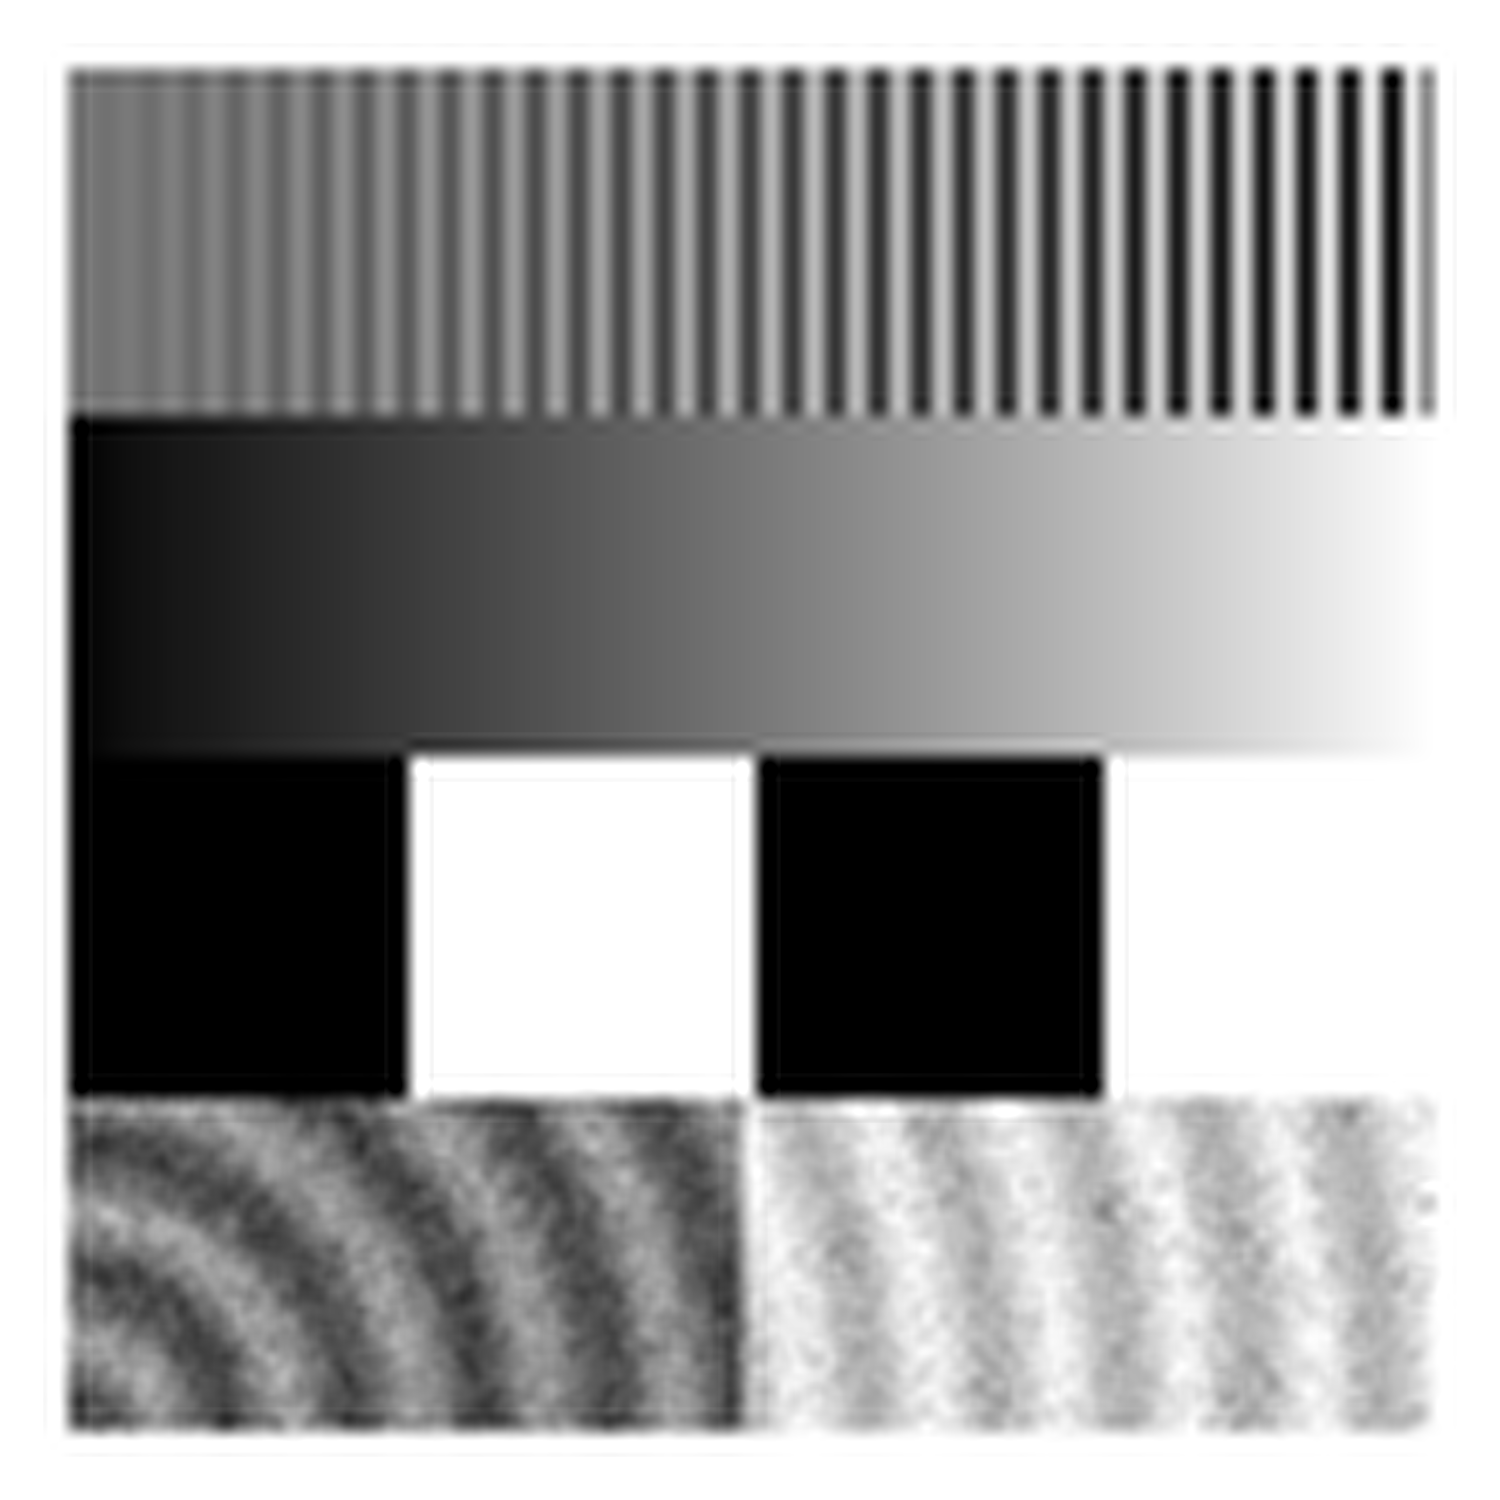
\includegraphics[width=.24\textwidth]{../imgs/savgol51_5} 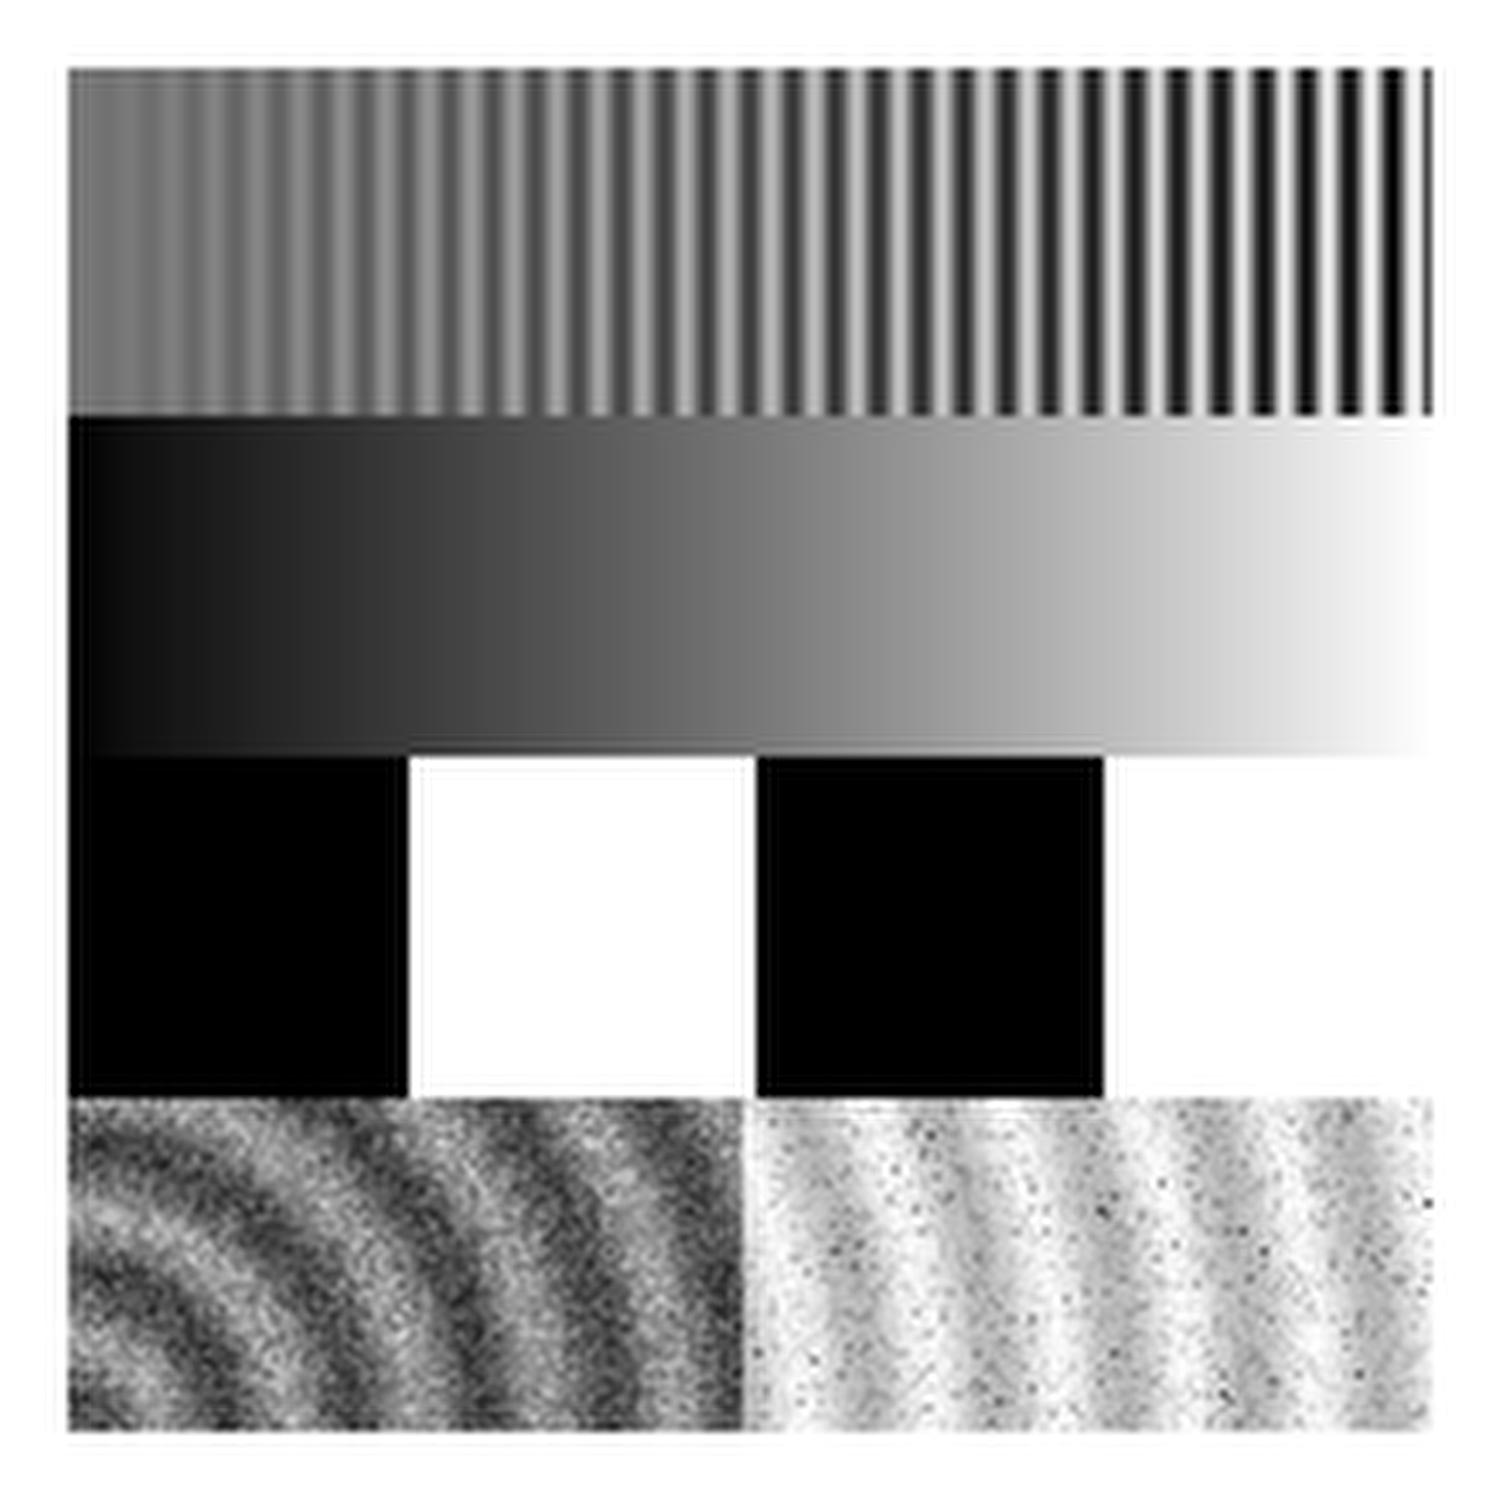
\includegraphics[width=.24\textwidth]{../imgs/savgol51_11} 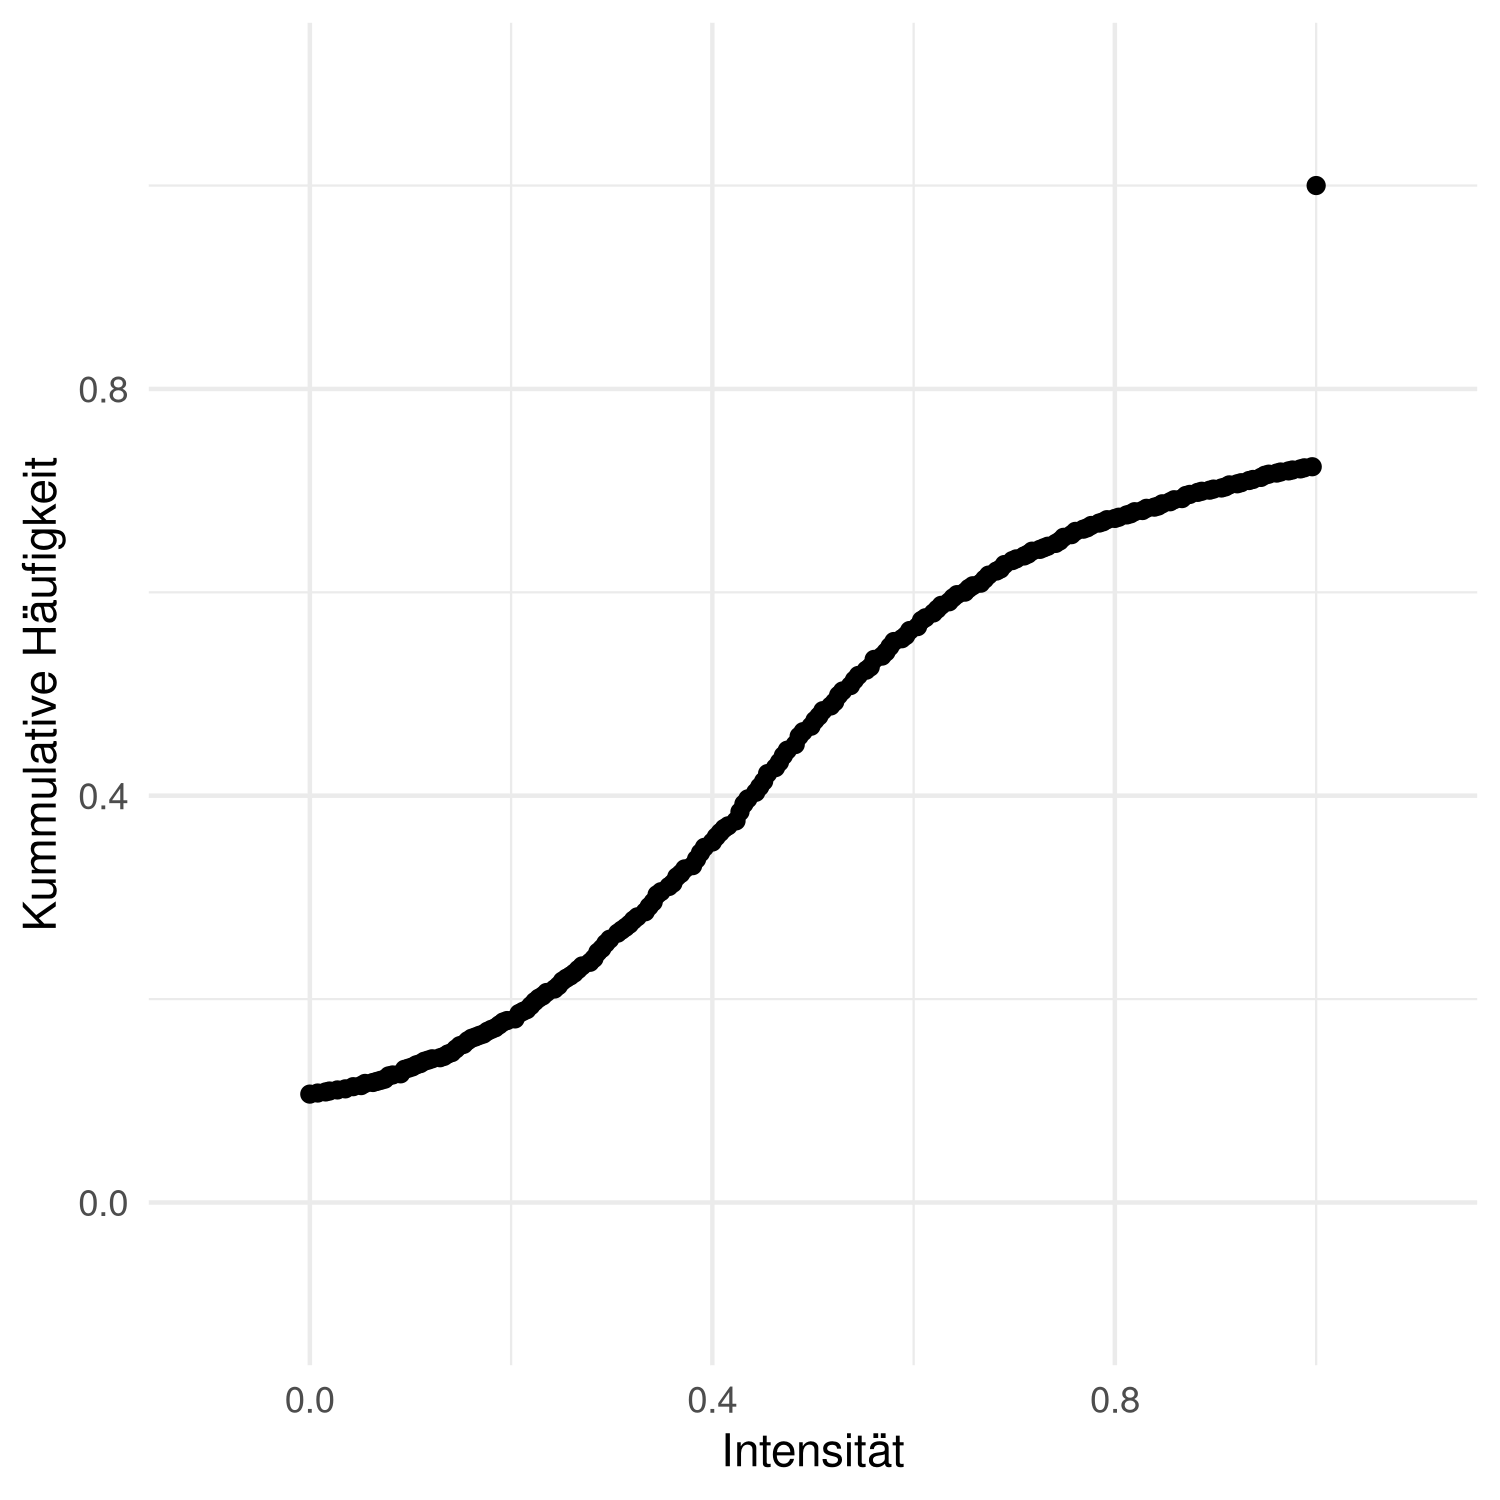
\includegraphics[width=.24\textwidth]{../imgs/hist_kum1} 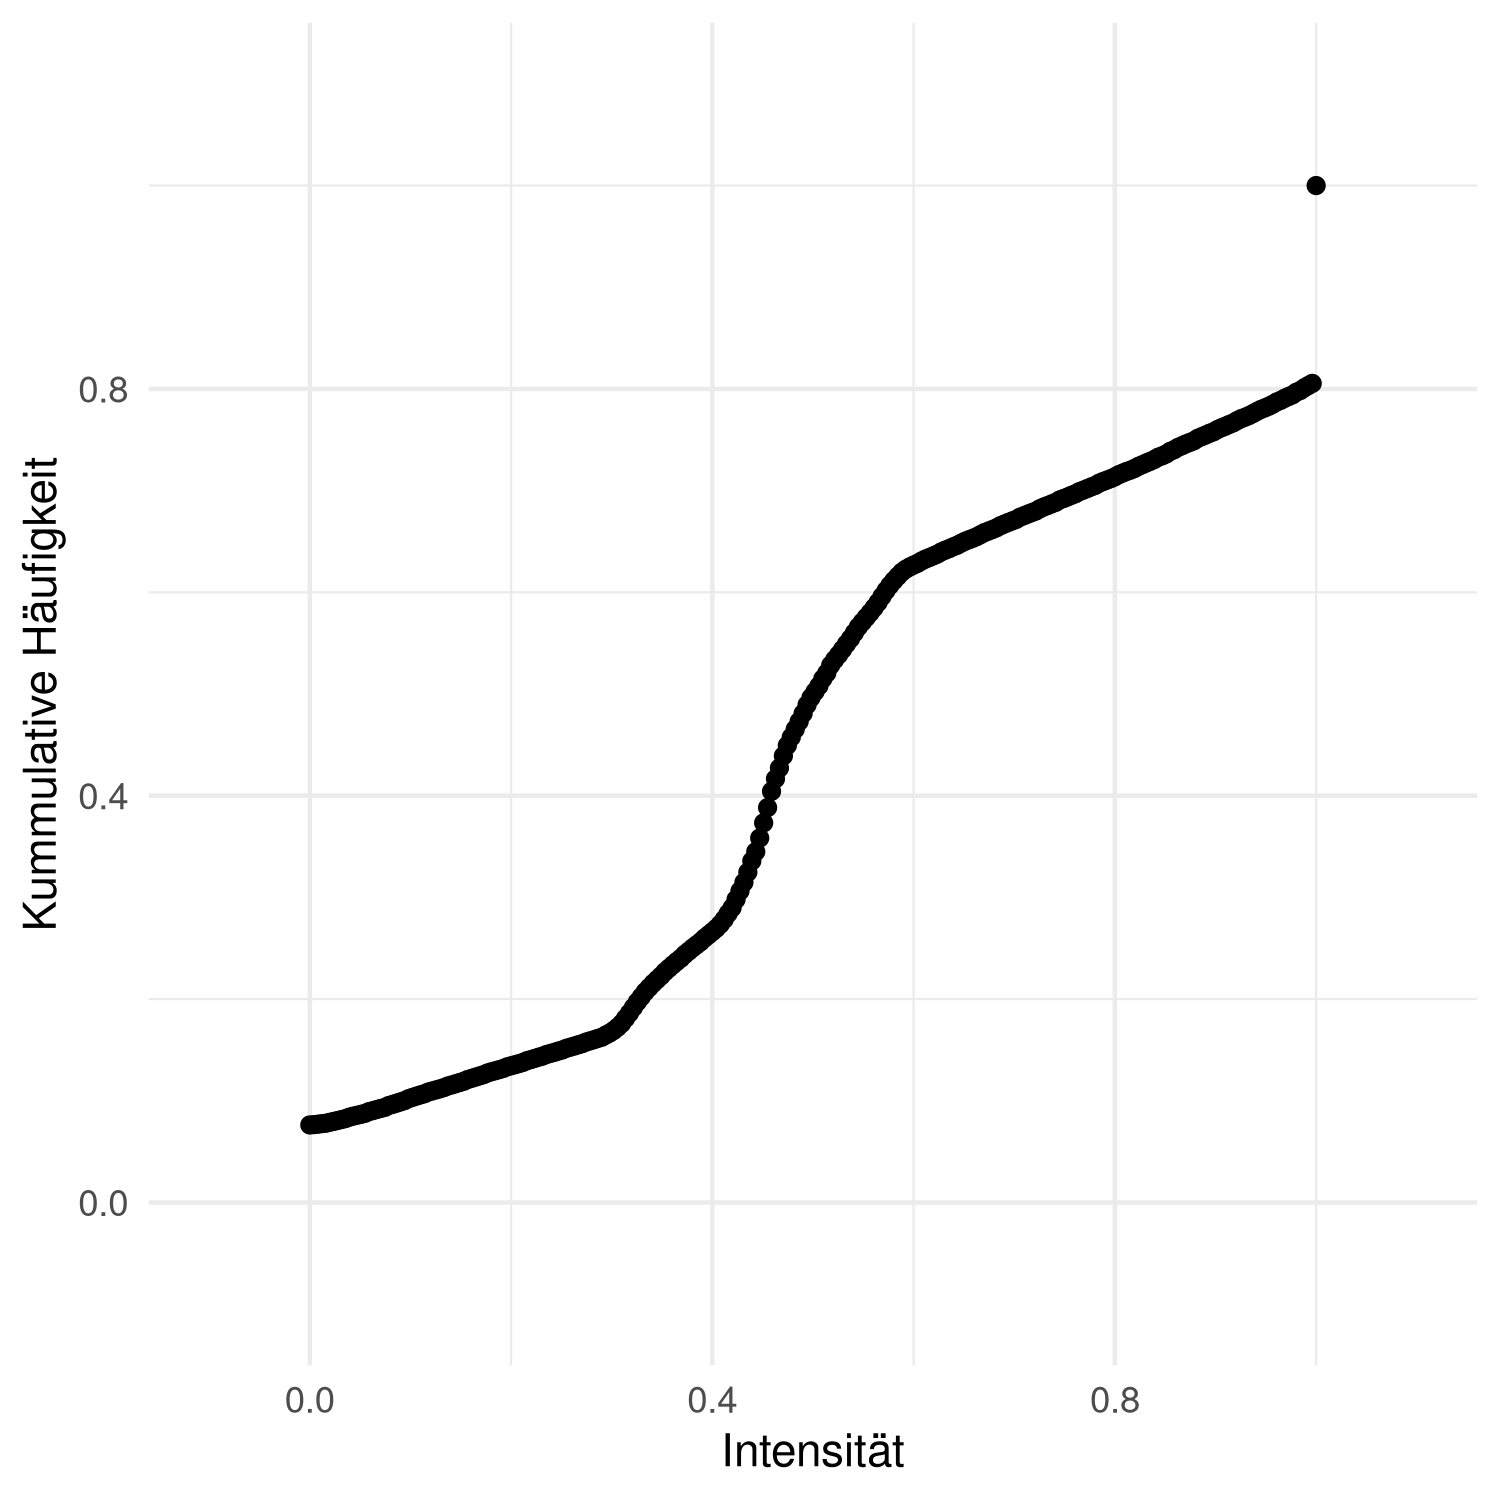
\includegraphics[width=.24\textwidth]{../imgs/savgol1} 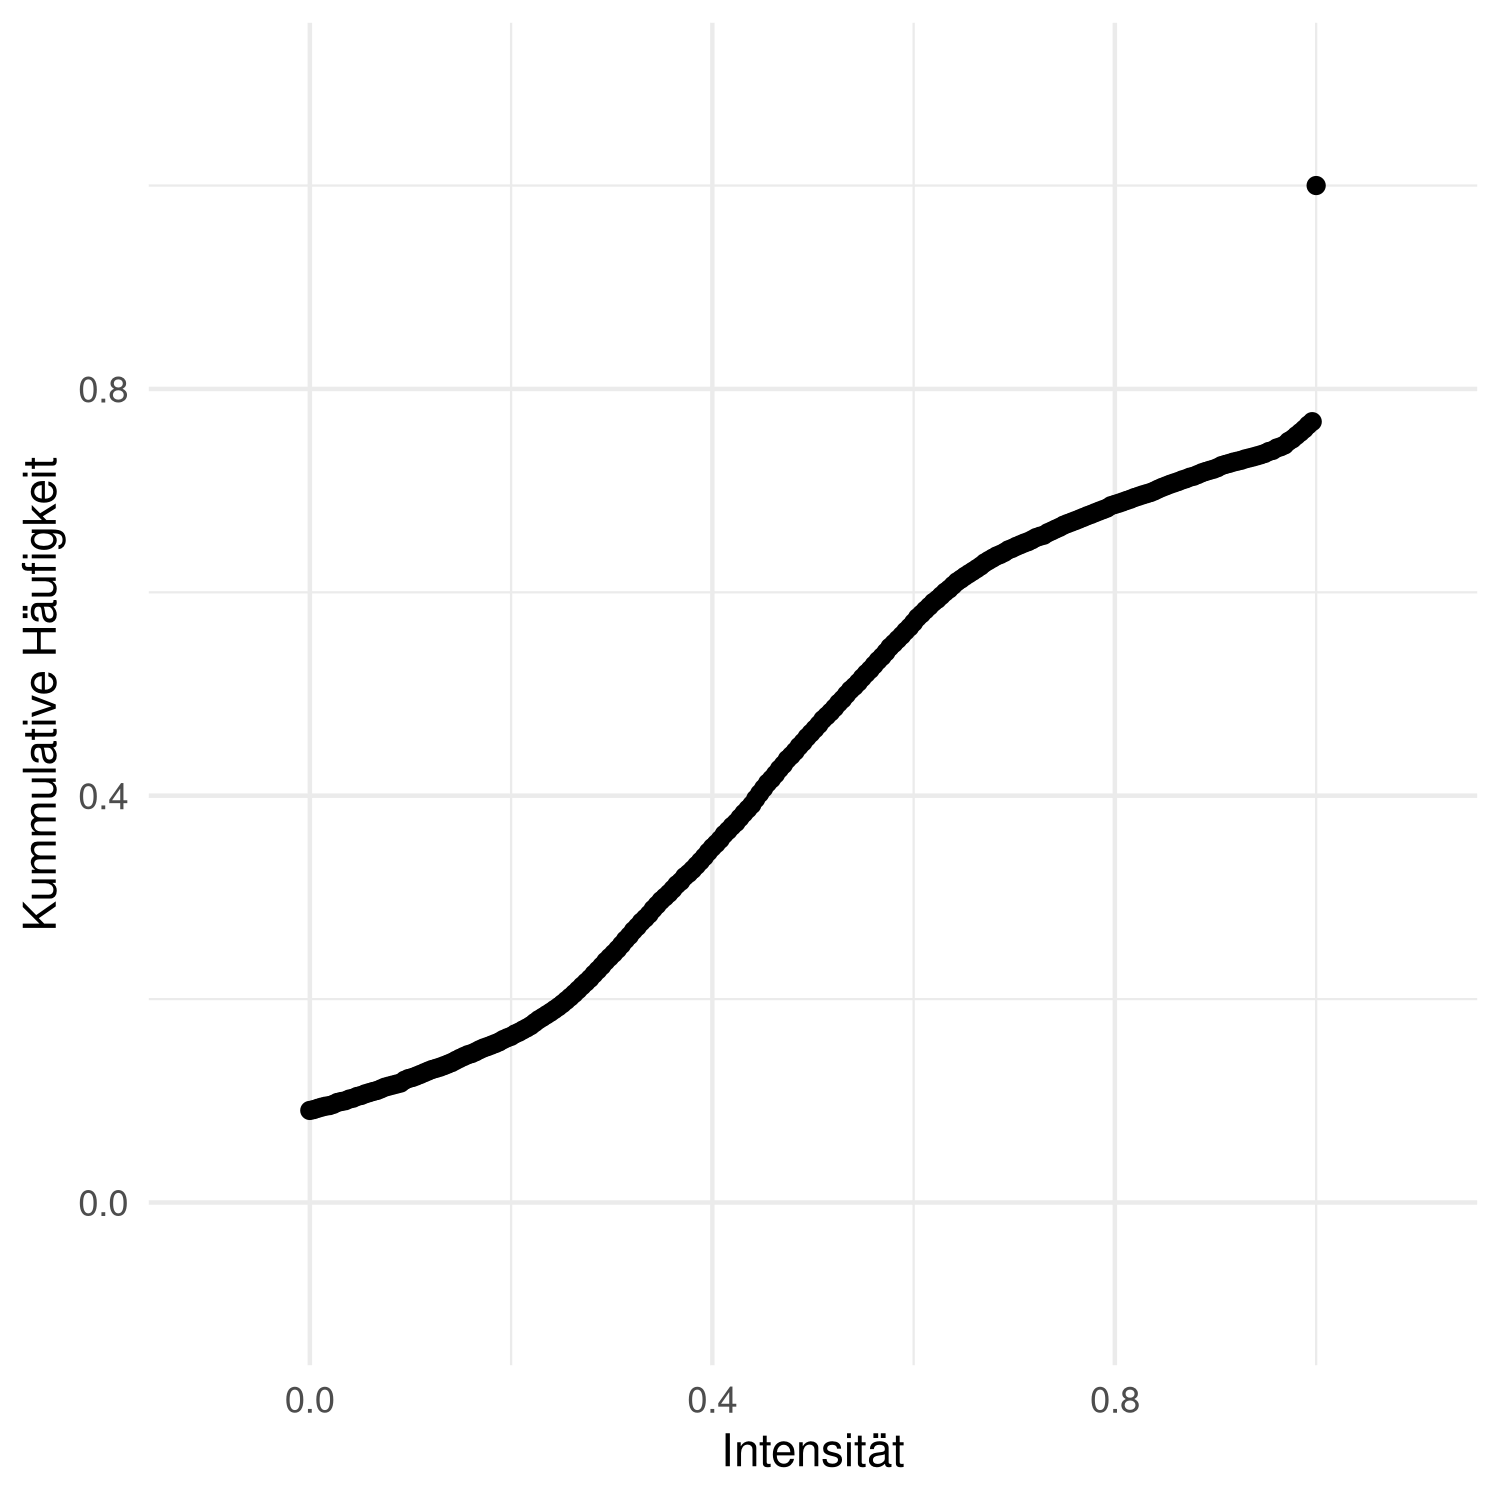
\includegraphics[width=.24\textwidth]{../imgs/savgol5} 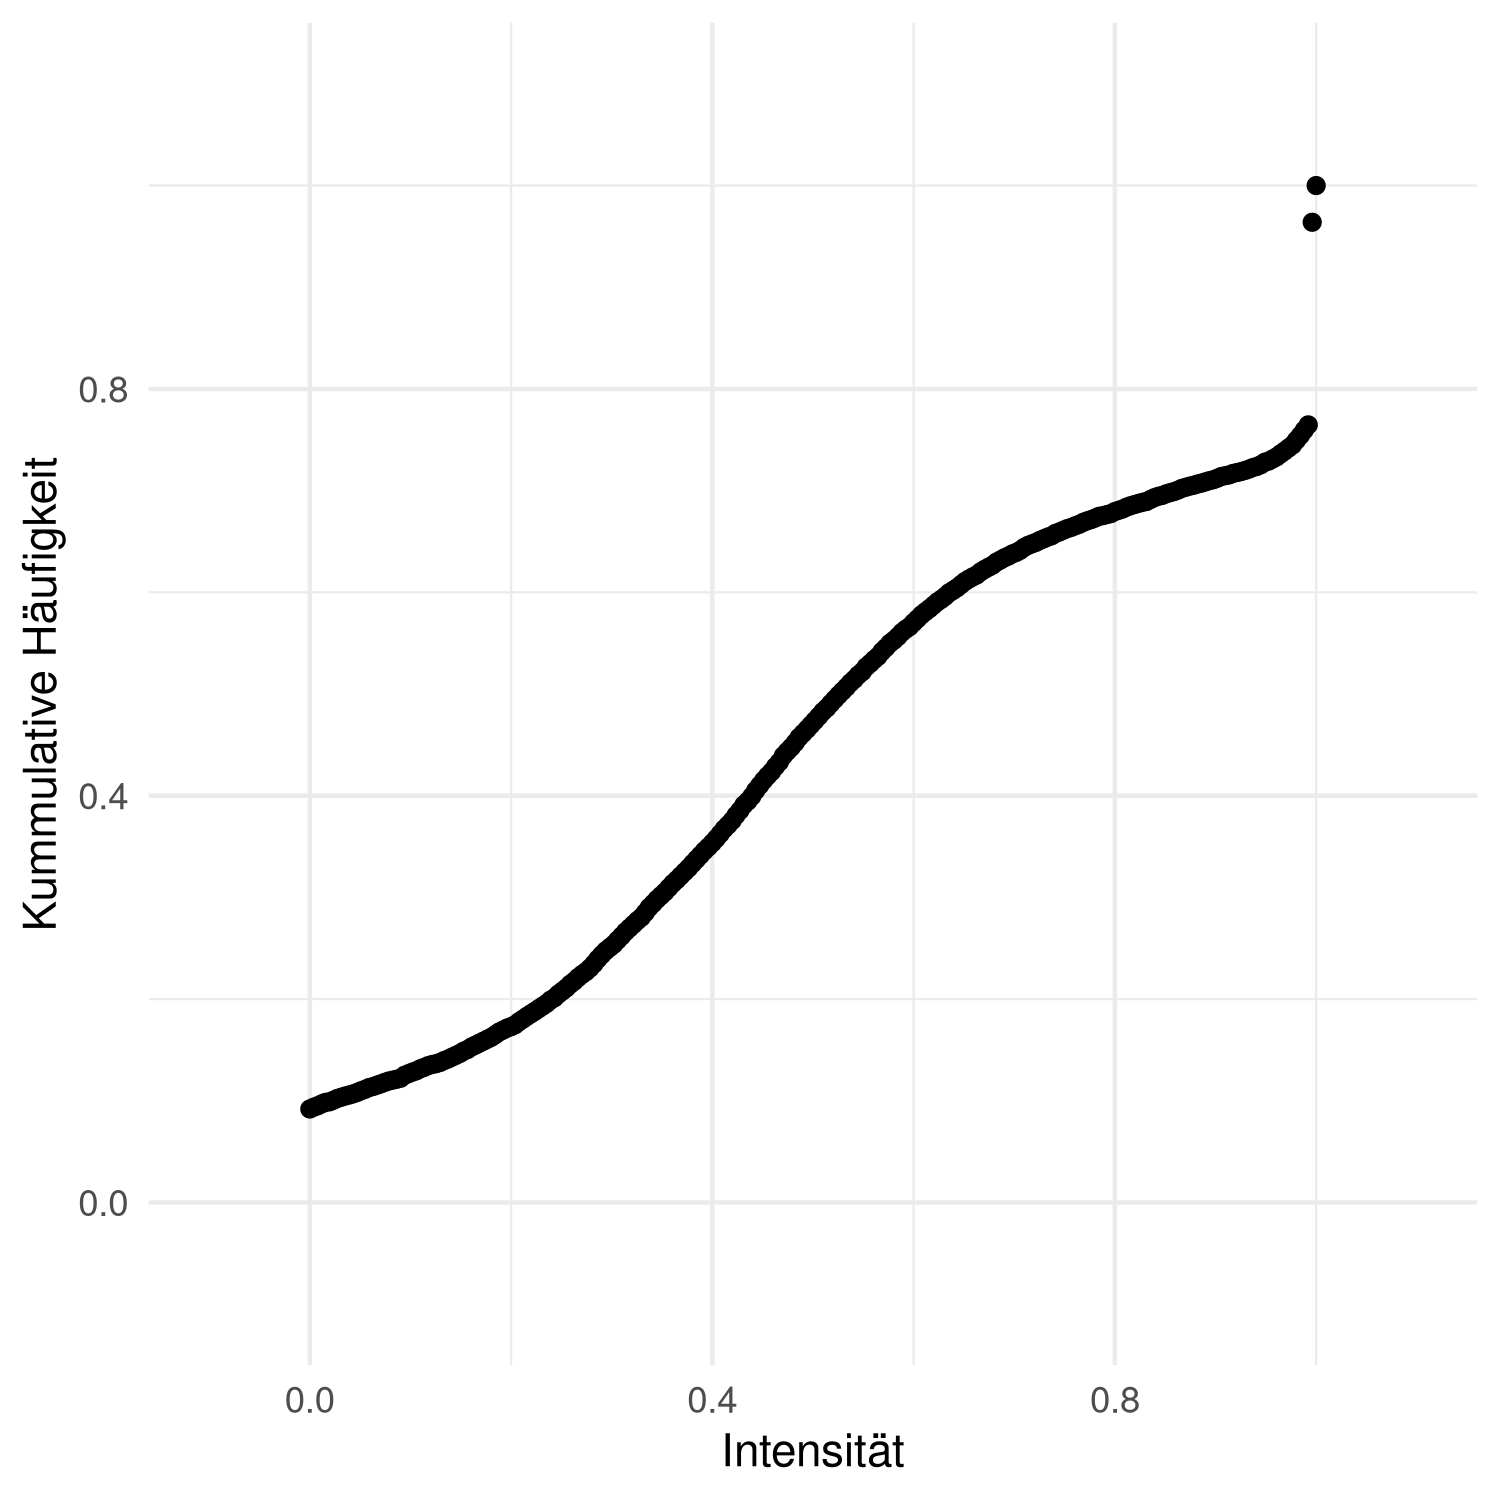
\includegraphics[width=.24\textwidth]{../imgs/savgol11} 

}

\caption[Beispielhafte Darstellung eines Savitzky-Golay-Filters.]{Beispielhafte Darstellung eines Savitzky-Golay-Filters. Links ist das Bild vor, rechts nach der Glättung der Helligkeitsverteilung zu sehen. Unten sind die Helligkeitsverteilungen abgebildet.}\label{fig:savgol}
\end{figure}

\hypertarget{bild-auswertung}{%
\section{Bild-Auswertung}\label{bild-auswertung}}

Der folgende Abschnitt beschäftigt sich mit den möglichen Ansätzen zur Erkennung der Kornflächen.
Für einen Überblick über Methoden zur Erkennung von Superpixeln und mögliche Architekturen zur Vermessung von Kornbildern.

\hypertarget{dbscan}{%
\subsection{DBSCAN}\label{dbscan}}

Der ursprünglich zur Gruppierung großer Datenbanken entwickelte Density-based Spatial Clustering of Applications with Noise (DBSCAN) Algorithmus (\protect\hyperlink{ref-esterIncrementalClusteringMining1998}{Ester et al., 1998}) konnte bereits erfolgreich zur Superpixel-Segmentierung in Echtzeit eingesetzt werden (\protect\hyperlink{ref-shenRealTimeSuperpixelSegmentation2016}{Shen et al., 2016}).

Der DBSCAN-Cluster-Algorithmus überprüft für jeden einzelnen Datenpunkt, wie viele Datenpunkte in einem vorgegebenen Radius oder \emph{epsilon} um den betrachteten Punkt liegen. Das Verfahren sortiert so Datenpunkt für Datenpunkt lokal über den Radius verknüpfte Einträge zusammen, die als zu einem Cluster zugehörig erklärt werden, sobald eine angegebene Mindestanzahl an Samples erreicht ist.

Durch das Schrittweise vorgehen bei diesem Verfahren, ist die Form der erkannten Cluster nicht festgelegt. Dadurch können auch komplexe Formen im Feature-Raum abgebildet wurden. Ein weiterer Vorteil ist die geringe Anfälligkeit für Ausreißer, da sich nicht im Radius um andere Punkte befindliche Datenpunkte einfach keinem Cluster zu sortiert werden.

In Abb. \ref{fig:dbscanExample} ist der Einfluss verschieden großer Radien und mindest-Clustergrößen dargestellt. Dazu ist jeweils die Laufzeit zur Erstellung der Clusterlösung abgetragen. Die Werte sind so skaliert, x- und y-Achse sowie die Farbwerte des ursprünglichen Bilds zwischen 0 und 100 liegen.





\begin{figure}

{\centering 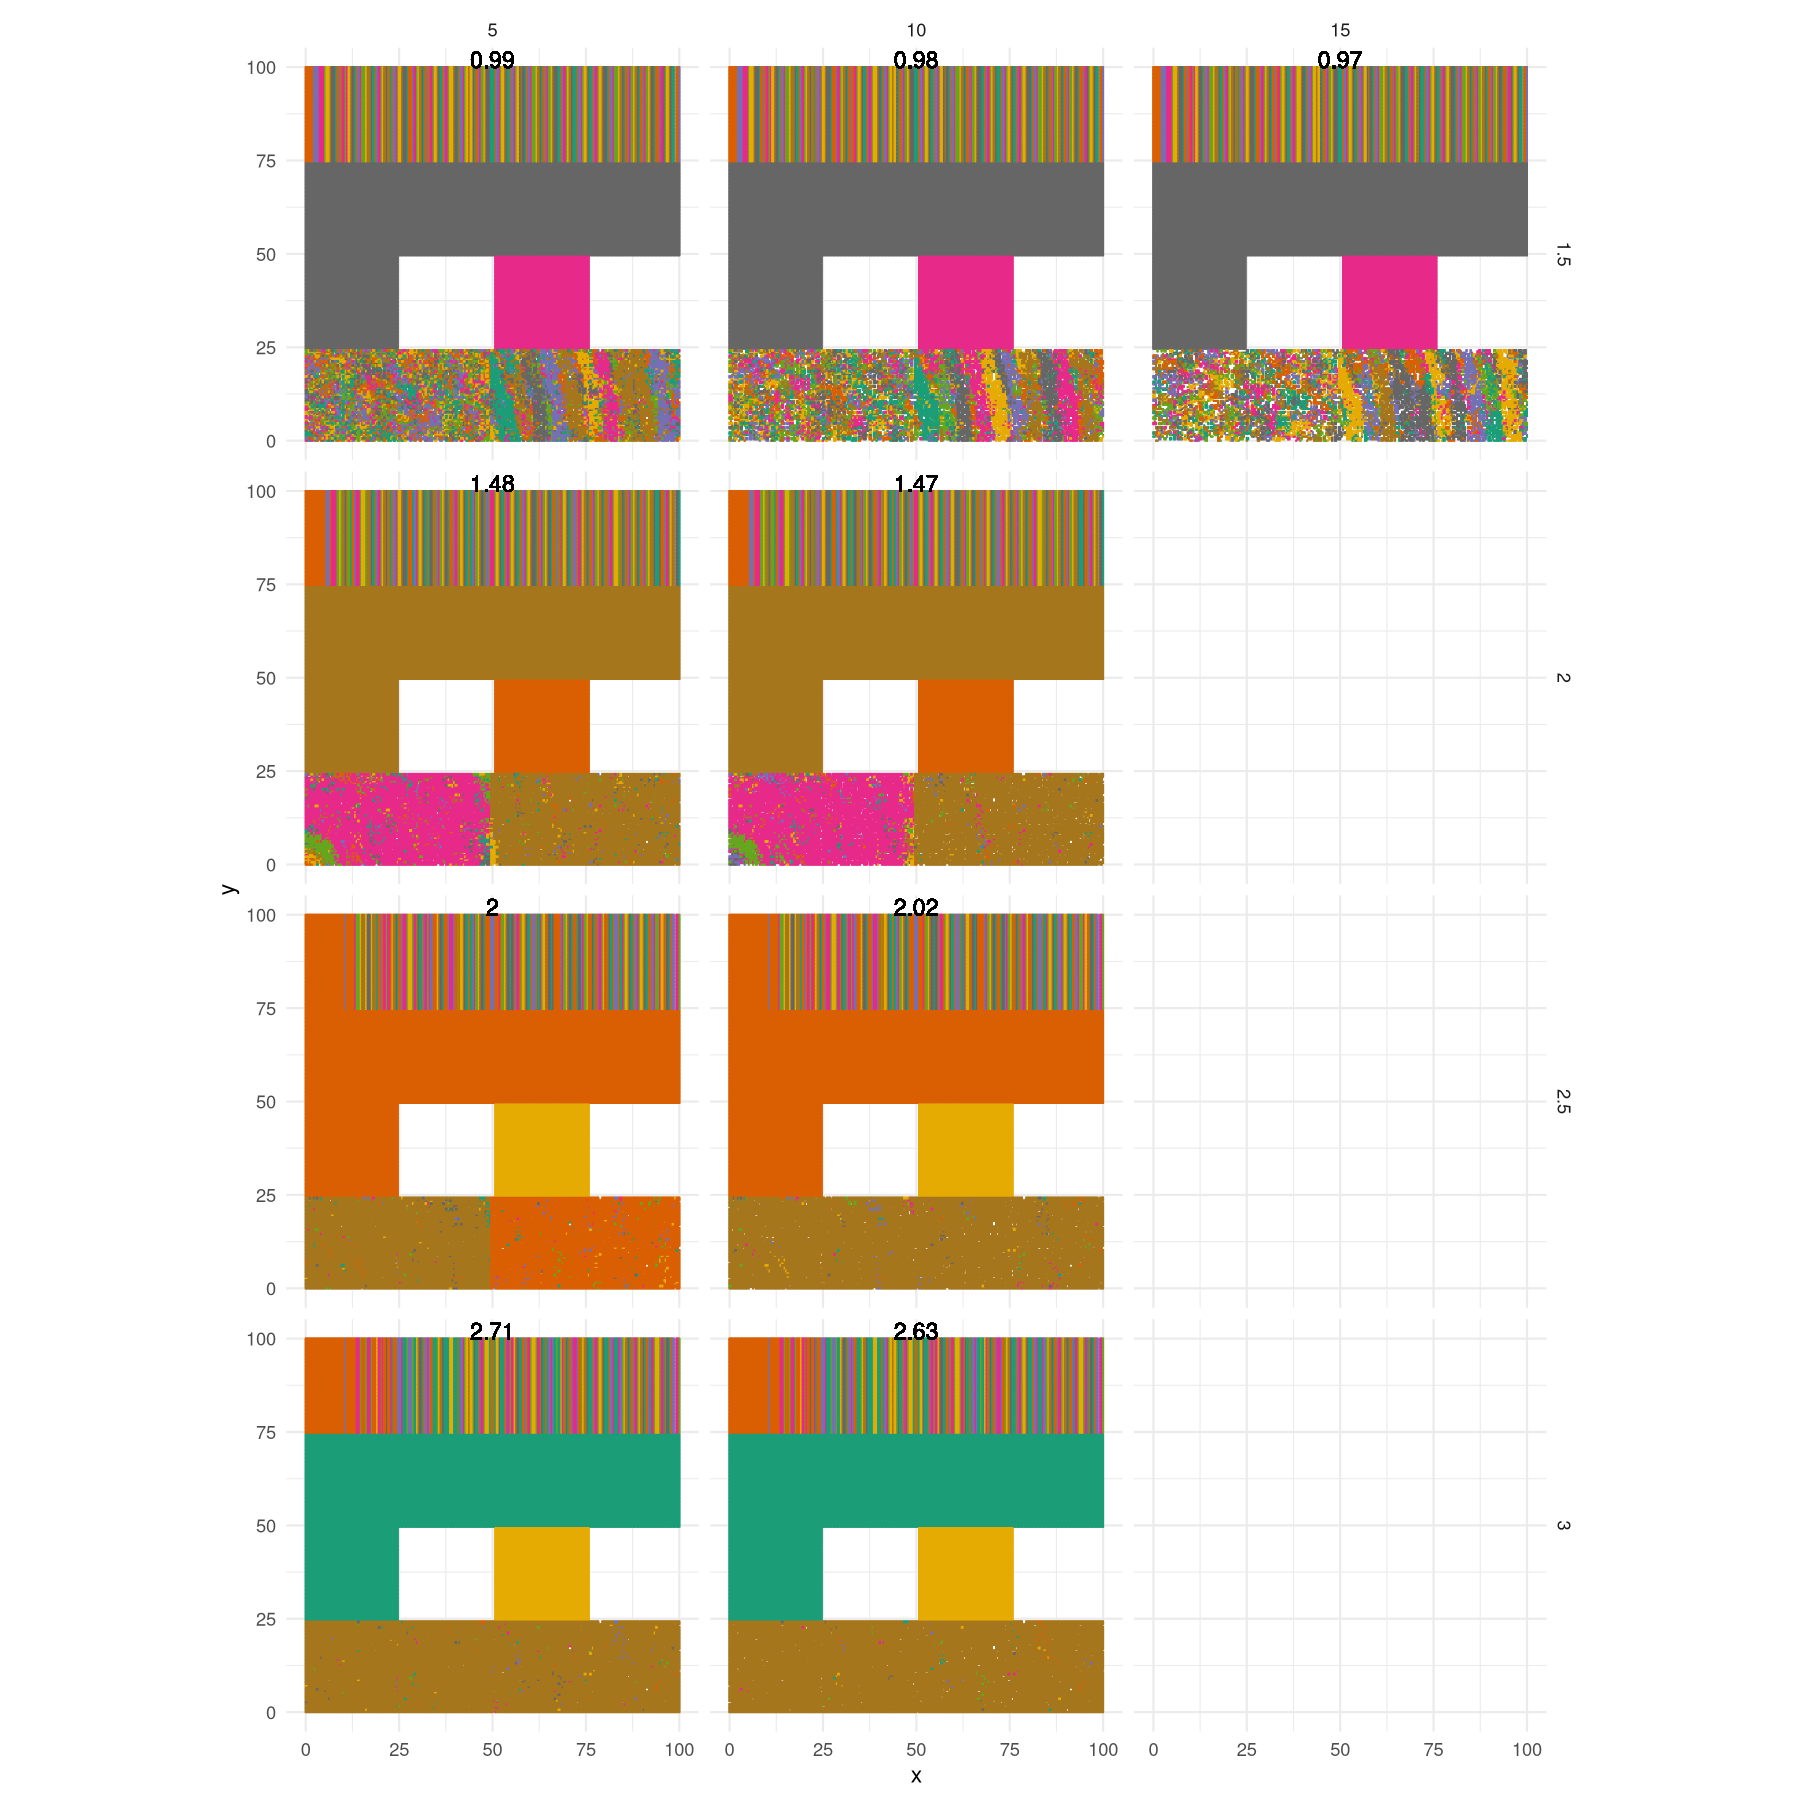
\includegraphics[width=0.96\textwidth]{../imgs/dbscan} 

}

\caption[Beispiel für Ergebnisse des DBSCAN-Algorithmus.]{Beispiel für Ergebnisse des DBSCAN-Algorithmus. Die Graphen stellen dasselbe Muster dar, farblich sind die erkannten Cluster eingefärbt. Mit jeder Zeile wird der betrachtete Radius, mit jeder Spalte die minimale Anzahl an Datenpunkten in einem Cluster erhöht. Die Werte sind so skaliert, x- und y-Achse sowie die Luminanzwerte des ursprünglichen Bilds zwischen 0 und 100 liegen. Die eingetragene Zahl ist die Dauer der Berechnung in Sekunden.}\label{fig:dbscanExample}
\end{figure}

\hypertarget{slic}{%
\subsection{SLIC}\label{slic}}

Beim als Superpixel-Segmentierungsansatz weit verbreiteten Simple Linear Iterative Clustering (SLIC) (\protect\hyperlink{ref-achantaSLICSuperpixelsCompared2012}{Achanta et al., 2012}) wird ein k-Means basiertes Verfahren genutzt, um näherungsweise gleich große Superpixel im Bild zu detektieren.
Dabei wird sowohl für den Farb- als auch den Pixelraum je eine euklidische Distanz aller Pixel zueinander berechnet, die dann gewichtet aufsummiert wird. Dabei wird in der Arbeit von Achanta et al. (\protect\hyperlink{ref-achantaSLICSuperpixelsCompared2012}{2012}) die räumliche Distanz gewichtet, wodurch mit hohen Werten des Hyperparameters \emph{m} die räumliche Nähe, mit niedrigen Werten die farbliche Nähe stärker gewichtet wird.

Der weitere Algorithmus ist im Prinzip der des normalen k-Means Clustering, das heißt Cluster-Kerne werden definiert (bei SLIC in regelmäßigen Abständen), Pixel werden den nächsten Clustern zugeordnet und die Zentroide dann auf die Zentroide der neuen Cluster verschoben.
Im Gegensatz zum regulären k-Means wird bei SLIC aber nicht im gesamten Datenraum nach möglichen Cluster-Angehörigen gesucht, sondern nur im doppelten Suchraum der vorgegebenen Clustergröße.
Achanta et al. (\protect\hyperlink{ref-achantaSLICSuperpixelsCompared2012}{2012}) beschreiben außerdem eine Adaptive Version des SLIC, bei dem die Cluster-Größe (und Anzahl) und die Gewichtung von räumlicher und farblicher Distanz Clusterweise angepasst wird, indem in jeder Iteration an der maximalen Distanz der vorhergehenden Iteration normalisiert wird.
In \ref{fig:slicExample} ist ein Beispiel für den ASLIC-Algorithmus mit unterschiedlichen \emph{m}-Gewichten und anfänglicher Cluster-Anzahl zu sehen.





\begin{figure}

{\centering 
\includegraphics[width=0.48\textwidth]{../imgs/slic_5_250} 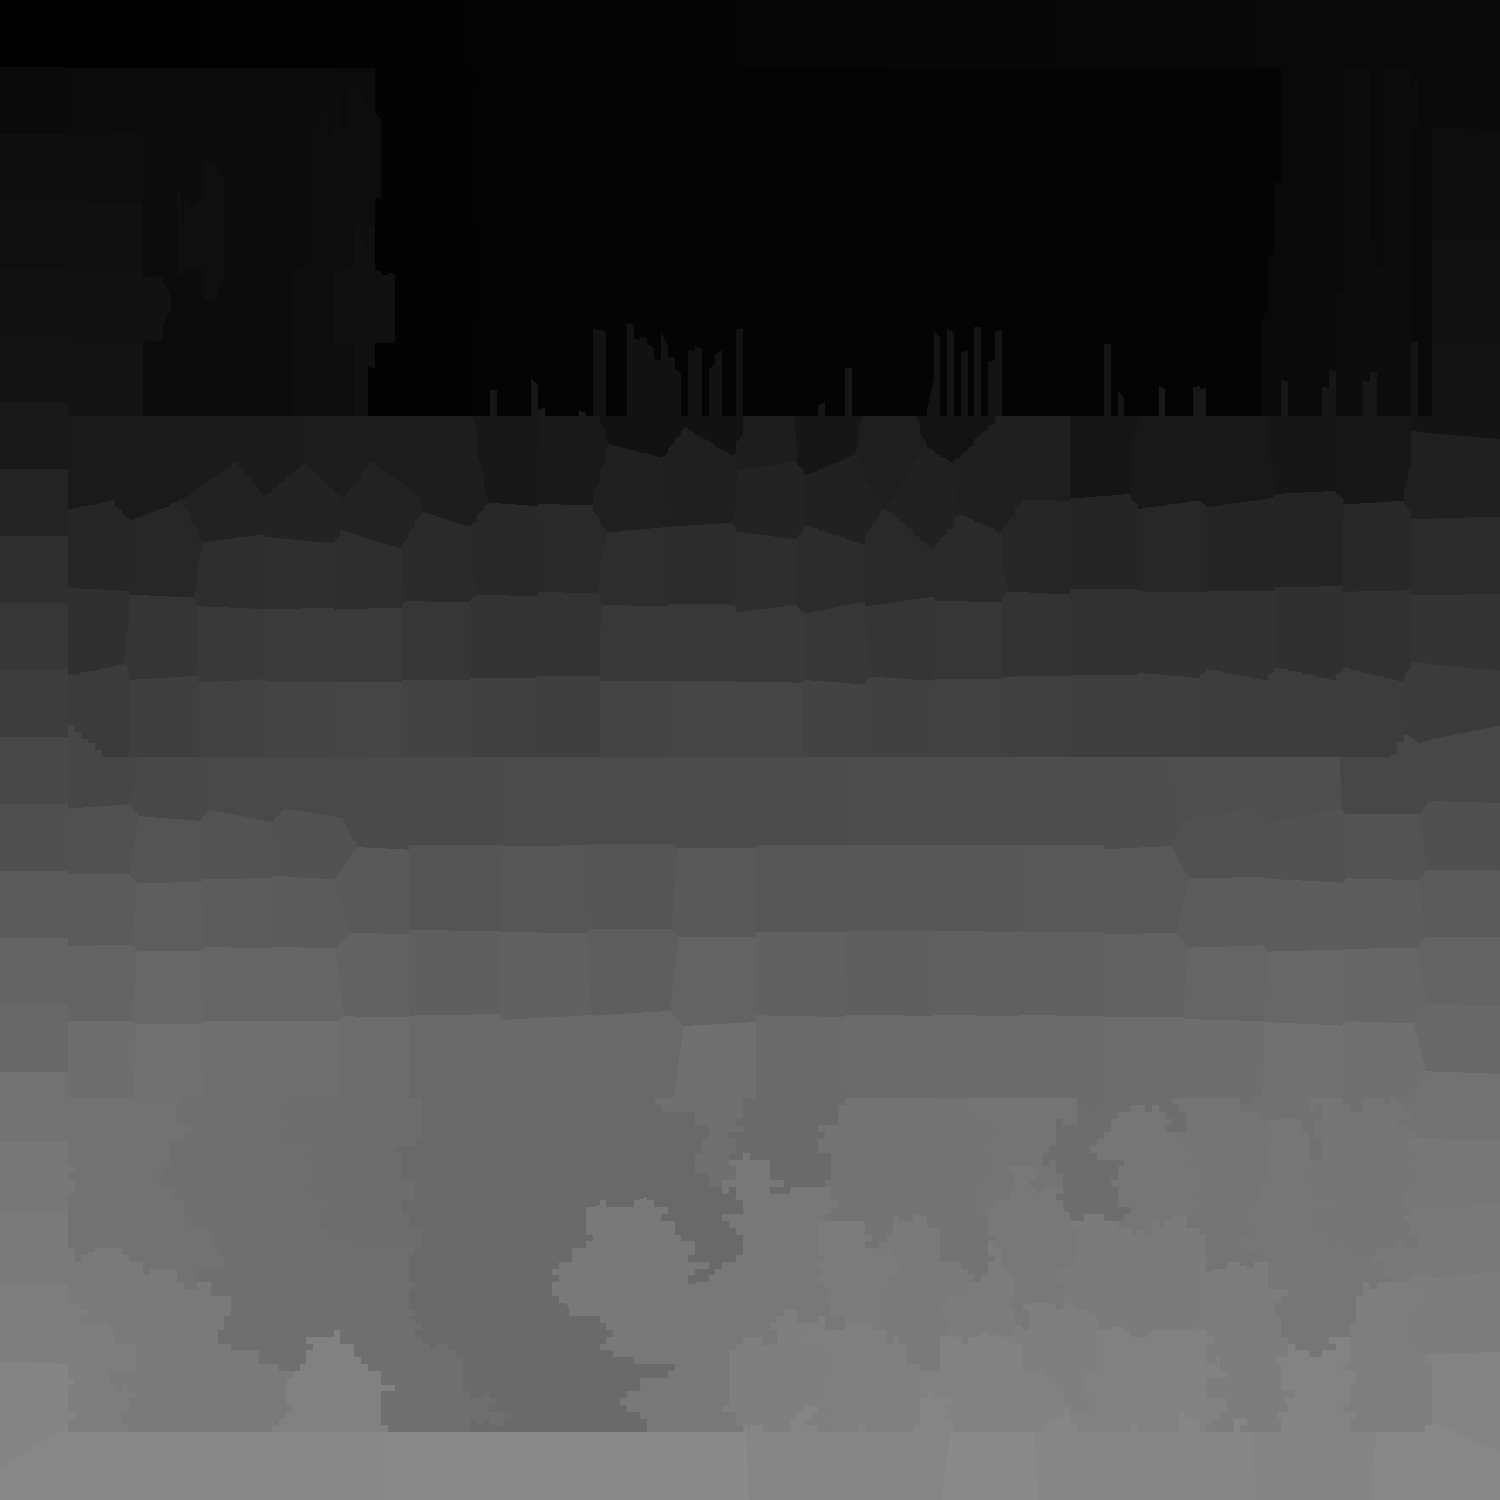
\includegraphics[width=0.48\textwidth]{../imgs/slic_5_500} 
\includegraphics[width=0.48\textwidth]{../imgs/slic_200_250} 
\includegraphics[width=0.48\textwidth]{../imgs/slic_200_500} 

}

\caption[Beispiel für eine Superpixel-Segmentierung mit SLIC.]{Beispiel für eine Superpixel-Segmentierung mit SLIC. Dargestellt sind die Cluster-Label als Grauschattierung. Links ist die Segmentierung mit 250 Start-Cluster-Zentren, rechts mit 500 dargestellt, oben je mit .1, unten mit 2 als Wert für \emph{m} zu sehen. In beiden Beispielen wurde die Adaptive Version des SLIC-Algorithmus wie bei Achanta et al. (\protect\hyperlink{ref-achantaSLICSuperpixelsCompared2012}{2012}) beschrieben eingesetzt.}\label{fig:slicExample}
\end{figure}

\hypertarget{normalized-cuts}{%
\subsection{Normalized Cuts}\label{normalized-cuts}}

Beim Normalized Cuts Verfahren zur Extraktion von Superpixeln (\protect\hyperlink{ref-shiNormalizedCutsImage2000}{Shi \& Malik, 2000}) wird das Bild in einen Graphen übersetzt, bei dem jeder Pixel durch einen Knoten repräsentiert wird. Jeder dieser Knoten wird dann mit jedem anderen Knoten über eine Kante verbunden, die über ein Maß gewichtet wird, das die Wahrscheinlichkeit der ``Zugehörigkeit zu einem Objekt'' (\protect\hyperlink{ref-shiNormalizedCutsImage2000}{Shi \& Malik, 2000}) ausdrückt.
Im Orginal-Paper wird die Wahrscheinlichkeit durch eine gewichtete Exponential-Funktion mit den Kontrastwerte und den geometrischen Distanzen im Exponenten ausgedrückt. Für beide Werte ist je eine Gewichtung vorgesehen, die angepasst werden kann - außerdem ein maximal zu berücksichtigender Radius für den geometrischen Abstand.

Unabhängig von der genauen Gewichtung der Kanten wird anschließend derjenige Schnitt gesucht, der die geringste Summe an Kantengewichten ``durchtrennt''. Dieser \emph{Normalized Cut} wird so bestimmt, dass die durch den Schnitt getrennten Gruppen möglichst unterschiedlich und die verbleibenden Gruppen in sich möglichst homogen sind. Die Lösung dieses Problem für ein ganzes Bild kann sehr aufwendig sein, weswegen zur Optimierung nur im geometrischen Umfeld der betrachteten Nodes gesucht wird.
Statt die Kanten mit der Wahrscheinlichkeits-Formel aus dem Papier von Shi \& Malik (\protect\hyperlink{ref-shiNormalizedCutsImage2000}{2000}) zu gewichten, können auch beliebige andere Gewichte gesetzt werden. So ist in der Implementation von NCuts, die in der Dokumentation des scikit-image-Python-Moduls(\protect\hyperlink{ref-NormalizedCutSkimage}{\emph{Normalized {Cut} --- Skimage V0.20.0.Dev0 Docs}, n.d.}) präsentiert wird, der Graph mit den Ergebnissen einer SLIC-Voranalyse gewichtet. Vor allem bei großen Bildern wird die von Shi \& Malik (\protect\hyperlink{ref-shiNormalizedCutsImage2000}{2000}) präsentierte Berechnung nahezu unmöglich, ohne große Optimierung ist allein eine Ergebnis-Matrix mit mindestens \(N_{Pixel}^2\over{2}\) Einträgen nötig.
Da SLIC aber in gewisser Form auch eine ``Wahrscheinlichkeit der Zugehörigkeit zum selben Objekt'' abdeckt, ist die Vorverarbeitung in diesem Sinne nicht wirklich gegen den intendierten Einsatz von NCuts.

\ref{fig:ncutsClassic}





\hypertarget{section}{%
\subsection{}\label{section}}

\hypertarget{bayesian-optimization-and-hyperband}{%
\subsection{Bayesian Optimization and Hyperband}\label{bayesian-optimization-and-hyperband}}

Nicht analytisch lösbare Optimierungsprobleme, insbesondere Hyperparameter-Auswahl, stellen einen zentralen Bestandteil der Data Science dar.

\hypertarget{literatur}{%
\chapter{Literatur}\label{literatur}}

\hypertarget{refs}{}
\begin{CSLReferences}{1}{0}
\leavevmode\vadjust pre{\hypertarget{ref-abouelattaClassificationCopperAlloys2013}{}}%
Abouelatta, O. B. (2013). Classification of copper alloys microstructure using image processing and neural network. \emph{Journal of American Science}, \emph{9}(6), 213--223.

\leavevmode\vadjust pre{\hypertarget{ref-achantaSLICSuperpixelsCompared2012}{}}%
Achanta, R., Shaji, A., Smith, K., Lucchi, A., Fua, P., \& Süsstrunk, S. (2012). {SLIC} superpixels compared to state-of-the-art superpixel methods. \emph{IEEE Transactions on Pattern Analysis and Machine Intelligence}, \emph{34}(11), 2274--2282.

\leavevmode\vadjust pre{\hypertarget{ref-akersRapidFlexibleSegmentation2021}{}}%
Akers, S., Kautz, E., Trevino-Gavito, A., Olszta, M., Matthews, B. E., Wang, L., Du, Y., \& Spurgeon, S. R. (2021). Rapid and flexible segmentation of electron microscopy data using few-shot machine learning. \emph{Npj Computational Materials}, \emph{7}(1, 1), 1--9. \url{https://doi.org/10.1038/s41524-021-00652-z}

\leavevmode\vadjust pre{\hypertarget{ref-ananyevCuGdCodoped2014}{}}%
Ananyev, M., Medvedev, D., Gavrilyuk, A., Mitri, S., Demin, A., Malkov, V., \& Tsiakaras, P. (2014). Cu and {Gd} co-doped {BaCeO3} proton conductors: {Experimental} vs {SEM} image algorithmic-segmentation results. \emph{Electrochimica Acta}, \emph{125}, 371--379. \url{https://doi.org/10.1016/j.electacta.2013.12.161}

\leavevmode\vadjust pre{\hypertarget{ref-askelandMaterialwissenschaftenGrundlagenUbungen1996}{}}%
Askeland, D. R. (1996). \emph{Materialwissenschaften: {Grundlagen}, {Übungen}, {Lösungen}}. {Spektrum Akad. Verlag}.

\leavevmode\vadjust pre{\hypertarget{ref-basuGaussianbasedEdgedetectionMethodsa2002}{}}%
Basu, M. (2002). Gaussian-based edge-detection methods-a survey. \emph{IEEE Transactions on Systems, Man, and Cybernetics, Part C (Applications and Reviews)}, \emph{32}(3), 252--260. \url{https://doi.org/10.1109/TSMCC.2002.804448}

\leavevmode\vadjust pre{\hypertarget{ref-buadesNonLocalMeansDenoising2011}{}}%
Buades, A., Coll, B., \& Morel, J.-M. (2011). Non-{Local Means Denoising}. \emph{Image Processing On Line}, \emph{1}, 208--212. \url{https://doi.org/10.5201/ipol.2011.bcm_nlm}

\leavevmode\vadjust pre{\hypertarget{ref-decostHighThroughputQuantitative2019}{}}%
DeCost, B. L., Lei, B., Francis, T., \& Holm, E. A. (2019). High {Throughput Quantitative Metallography} for {Complex Microstructures Using Deep Learning}: {A Case Study} in {Ultrahigh Carbon Steel}. \emph{Microscopy and Microanalysis}, \emph{25}(1), 21--29. \url{https://doi.org/10.1017/S1431927618015635}

\leavevmode\vadjust pre{\hypertarget{ref-dengizGrainBoundaryDetection2005}{}}%
Dengiz, O., Smith, A. E., \& Nettleship, I. (2005). Grain boundary detection in microstructure images using computational intelligence. \emph{Computers in Industry}, \emph{56}(8-9), 854--866. \url{https://doi.org/10.1016/j.compind.2005.05.012}

\leavevmode\vadjust pre{\hypertarget{ref-esterIncrementalClusteringMining1998}{}}%
Ester, M., Kriegel, H.-P., Sander, J., Wimmer, M., \& Xu, X. (1998). Incremental {Clustering} for {Mining} in a {Data Warehousing Environment}. \emph{Proceedings of the 24rd {International Conference} on {Very Large Data Bases}}, 323--333.

\leavevmode\vadjust pre{\hypertarget{ref-GefugeWerkstoffkunde2021}{}}%
Gefüge (Werkstoffkunde). (2021). In \emph{Wikipedia}. \url{https://de.wikipedia.org/w/index.php?title=Gef\%C3\%BCge_(Werkstoffkunde)\&oldid=214385861}

\leavevmode\vadjust pre{\hypertarget{ref-harishvijeyAutomatedTechniqueEEG2022}{}}%
Harishvijey, A., \& Benadict Raja, J. (2022). Automated technique for {EEG} signal processing to detect seizure with optimized {Variable Gaussian Filter} and {Fuzzy RBFELM} classifier. \emph{Biomedical Signal Processing and Control}, \emph{74}, 103450. \url{https://doi.org/10.1016/j.bspc.2021.103450}

\leavevmode\vadjust pre{\hypertarget{ref-heilbronnerAutomaticGrainBoundary2000}{}}%
Heilbronner, R. (2000). Automatic grain boundary detection and grain size analysis using polarization micrographs or orientation images. \emph{Journal of Structural Geology}, \emph{22}(7), 969--981. \url{https://doi.org/10.1016/S0191-8141(00)00014-6}

\leavevmode\vadjust pre{\hypertarget{ref-heynShortReportsMetallurgical1903}{}}%
Heyn, E. (1903). Short reports from the metallurgical and metallographical laboratory of the royal mechanical and technical testing institute of charlottenburg. \emph{The Metallographist}, \emph{5}, 39--64.

\leavevmode\vadjust pre{\hypertarget{ref-kimUnsupervisedMicrostructureSegmentation2020}{}}%
Kim, H., Inoue, J., \& Kasuya, T. (2020). Unsupervised microstructure segmentation by mimicking metallurgists' approach to pattern recognition. \emph{Scientific Reports}, \emph{10}(1, 1), 17835. \url{https://doi.org/10.1038/s41598-020-74935-8}

\leavevmode\vadjust pre{\hypertarget{ref-kitagawaTwofilterFormulaSmoothing1994}{}}%
Kitagawa, G. (1994). The two-filter formula for smoothing and an implementation of the {Gaussian-sum} smoother. \emph{Annals of the Institute of Statistical Mathematics}, \emph{46}(4), 605--623.

\leavevmode\vadjust pre{\hypertarget{ref-latifDeepLearningBasedAutomaticMineral2022}{}}%
Latif, G., Bouchard, K., Maitre, J., Back, A., \& Bédard, L. P. (2022). Deep-{Learning-Based Automatic Mineral Grain Segmentation} and {Recognition}. \emph{Minerals}, \emph{12}(4, 4), 455. \url{https://doi.org/10.3390/min12040455}

\leavevmode\vadjust pre{\hypertarget{ref-liMetallographicImageSegmentation2020}{}}%
li, M., Chen, D., Liu, S., \& Liu, F. (2020). Metallographic {Image Segmentation Method Based} on {Superpixels Algorithm} and {Transfer Learning}. \emph{2020 {Chinese Control And Decision Conference} ({CCDC})}, 1922--1926. \url{https://doi.org/10.1109/CCDC49329.2020.9164466}

\leavevmode\vadjust pre{\hypertarget{ref-maitreMineralGrainsRecognition2019}{}}%
Maitre, J., Bouchard, K., \& Bédard, L. P. (2019). Mineral grains recognition using computer vision and machine learning. \emph{Computers \& Geosciences}, \emph{130}, 84--93. \url{https://doi.org/10.1016/j.cageo.2019.05.009}

\leavevmode\vadjust pre{\hypertarget{ref-MetallographieRostfreiemStahl}{}}%
\emph{Metallographie von rostfreiem {Stahl}}. (n.d.). Retrieved December 14, 2021, from \url{https://www.struers.com/de-DE/Knowledge/Materials/Stainless-Steel\#etching}

\leavevmode\vadjust pre{\hypertarget{ref-NormalizedCutSkimage}{}}%
\emph{Normalized {Cut} --- skimage v0.20.0.Dev0 docs}. (n.d.). Retrieved June 23, 2022, from \url{https://scikit-image.org/docs/dev/auto_examples/segmentation/plot_ncut.html?highlight=normalization}

\leavevmode\vadjust pre{\hypertarget{ref-offentlichkeitsarbeitPersonalGeorgAugustUniversitatGottingen}{}}%
Öffentlichkeitsarbeit, G.-A.-U. G.-. (n.d.-a). \emph{Personal - Georg-August-Universität Göttingen}. Retrieved May 9, 2022, from \url{https://www.uni-goettingen.de/de/652520.html}

\leavevmode\vadjust pre{\hypertarget{ref-offentlichkeitsarbeitStudiumUndLehre}{}}%
Öffentlichkeitsarbeit, G.-A.-U. G.-. (n.d.-b). \emph{Studium und Lehre - Georg-August-Universität Göttingen}. Retrieved May 9, 2022, from \url{https://www.uni-goettingen.de/de/626487.html}

\leavevmode\vadjust pre{\hypertarget{ref-princePartIVPreprocessing2012}{}}%
Prince, S. J. (2012). Part {IV}: {Preprocessing}. In \emph{Computer vision: Models, learning, and inference} (pp. 321--354). {Cambridge University Press}.

\leavevmode\vadjust pre{\hypertarget{ref-shenRealTimeSuperpixelSegmentation2016}{}}%
Shen, J., Hao, X., Liang, Z., Liu, Y., Wang, W., \& Shao, L. (2016). Real-{Time Superpixel Segmentation} by {DBSCAN Clustering Algorithm}. \emph{IEEE Transactions on Image Processing}, \emph{25}(12), 5933--5942. \url{https://doi.org/10.1109/TIP.2016.2616302}

\leavevmode\vadjust pre{\hypertarget{ref-shiNormalizedCutsImage2000}{}}%
Shi, J., \& Malik, J. (2000). Normalized cuts and image segmentation. \emph{IEEE Transactions on Pattern Analysis and Machine Intelligence}, \emph{22}(8), 888--905. \url{https://doi.org/10.1109/34.868688}

\leavevmode\vadjust pre{\hypertarget{ref-StandardTestMethods2021}{}}%
\emph{Standard {Test Methods} for {Determining Average Grain Size}}. (2021, November 17). \url{https://www.astm.org/e0112-13.html}

\leavevmode\vadjust pre{\hypertarget{ref-wangSuperpixelSegmentationBenchmark2017}{}}%
Wang, M., Liu, X., Gao, Y., Ma, X., \& Soomro, N. Q. (2017). Superpixel segmentation: {A} benchmark. \emph{Signal Processing: Image Communication}, \emph{56}, 28--39. \url{https://doi.org/10.1016/j.image.2017.04.007}

\leavevmode\vadjust pre{\hypertarget{ref-winkDenoisingFunctionalMR2004}{}}%
Wink, A. M., \& Roerdink, J. B. (2004). Denoising functional {MR} images: A comparison of wavelet denoising and {Gaussian} smoothing. \emph{IEEE Transactions on Medical Imaging}, \emph{23}(3), 374--387.

\end{CSLReferences}

\end{document}
